\chapter{Transport}
\label{chap:transport}

\section{Introduction}
This chapter focuses on the transport scheme in a CTM. As illustrated in the
introduction (see Fig.~\ref{fig:chem_processes}), the transport is actually a
set of several processes: advection, turbulent diffusion, convection and
particles sedimentation. Some of these processes can be represented directly,
\textit{i.e.}, the model solves the corresponding equations to find the
evolution of the quantities over time. It is the case for advection, where
large-scale winds move the chemical species away from their sources, and for
particles sedimentation. Other processes are too complex to be represented
directly and a \textit{parametrization} is used to estimate their average impact
on the tracers inside the cells of a model. This is the case for turbulent
diffusion and convection as their spatial and temporal scales are too small for
the model.

% Change numbering back to default here as we need to cite the intro before
\renewcommand{\thefigure}{\arabic{chapter}.\arabic{figure}}

In this thesis, we focus on horizontal advection, which is a core process for
CTMs. It is especially important for our model as it serves as the framework for our
parallelization strategy (presented in Chapter~\ref{chap:parallel}). After
presenting key properties for an advection scheme in
Section~\ref{sec:properties}, we then give an overview of the different
numerical methods used in past and current transport schemes to solve the mass
and continuity equations for tracers (Section~\ref{sec:history}).  Mass
conservation is a key property in CTMs so we examine finite-volume schemes which
allow for local and global conservation. The description of the scheme chosen in
Pangolin follows.  A major drawback for finite-volume schemes and Eulerian
schemes is the "pole problem" on the traditional regular latitude-longitude
grid. Active research is currently performed on alternative grids to avoid this
issue. This issue, along with the current alternative grids that have been so
far studied to solve it, are presented in Section~\ref{subsec:grids}. Within
Pangolin, we introduce a new quasi-area preserving grid which maps uniformly the
sphere and alleviates the pole issue. The new grid is presented in
Section~\ref{subsec:pango_grid}, along with the necessary adaption of the
finite-volume scheme.

\section{Properties of the scheme}
\label{sec:properties}
Here, we examine desirable features of a transport scheme in atmospheric
applications. The first property is accuracy, which quantifies how close we are to
the exact solution in a given norm. There are several possibilities to define a
norm, but in practice, the most common norms are (see~\cite{Williamson1992}):
\def\II{\mathcal{I}}
\begin{equation}
  l_1 = \frac{\II(|q-q_E|)}{\II(|q_E|)}
  \qquad
  l_2 = \frac{\sqrt{\II((q-q_E)^2)}}{\sqrt{\II(q_E^2)}}
  \qquad
  l_\infty = \frac{\max |q-q_E|}{\max{|q_E|}},
  \label{eqn:err_norms}
\end{equation}
where $q$ is the tracer distribution (depending on space and time) and $q_E$ the
exact distribution. $\II$ is the integral of the distribution over the sphere.
Using these norms, we can compute an absolute error at a given resolution or the
error for several resolutions to examine the convergence rate. A formal order of
accuracy can also be obtained by using truncated Taylor series in the original
equations. After removing the cancelling terms, the lowest order term gives the
order of the scheme. However, it does not provide any guarantee about accuracy at
a given resolution, nor near discontinuities. For global models, the objective
is rather to decrease the error at a given resolution, rather than improving the
formal order of accuracy.  \\
Another issue is that exact solutions are not always available. In real-case
scenario, we only have access to the results of other models and observational
data. Observations are non-uniform in space and in time (every few hours in
practice). That is why a scheme is first tested on algebraic test cases
representative of atmospheric transport, where the algebraic solution is known.
Such tests are detailed in Chapter~\ref{chap:testing}. Once the model has been
validated on these test cases, "real" data can be used, as shown in
Chapter~\ref{chap:real_case}.

When choosing a numerical scheme, its stability should be examined carefully.
For Eulerian formulations, we typically have a \gls{CFL} condition restricting
the time-step to avoid numerical divergence during the simulation. On a regular
latitude-longitude grid, this condition severely restricts the time-step due to
the convergence of meridians at the pole. This issue led to different solutions, as
explained in Section~\ref{sec:history}. A related desirable feature is the
geometric flexibility, \textit{i.e}, how dependent it is on the grid.
Mass preservation is another important feature. If we consider the total dry air
mass in the atmosphere, there are only very small variations due to physical
processes so the lack of mass preservation leads to non-physical solutions. It is
also important to preserve the mass of long-lived tracers such as stratospheric
ozone. Highly reactive substances such as reactive chlorine must also preserve
the sum of their compound.

The equations to solve for the transport are the air mass and tracer mass
continuity equations\footnote{Vectors as written in bold.}:
\begin{align}
  &\frac{\partial \rho}{\partial t} + \nabla \cdot (\rho {\bf V}) = 0 ,
  \label{eqn:air}
  \\
  &\frac{\partial \rho q}{\partial t} + \nabla \cdot ( \rho q {\bf V})  = 0,
  \label{eqn:tracer}
\end{align}
where $\rho$ is the air density, $q$ the tracer mixing ratio and ${\bf V}$ the
winds vector field. If the grid and the time-step are identical for the air and
tracer transport, then the tracer transport should default to the air transport
when $q=1$. Otherwise, this can lead to spurious mass creation or
deletion, the so-called "mass-wind inconsistency". 

The transport scheme should preserve the shape of the tracer distribution. In
particular, the scheme should be range-preserving and positivity preserving. It
avoids negative ratio or ratio outside the physical range, which can cause
issues with the chemistry or parametrization later on. Spurious extrema should
also be avoided (monotonicity constraint). Also, the scheme
should be non-oscillatory, meaning large gradients should not create "wiggles"
in the distribution.

When advecting several tracers, the transport scheme should preserve the
different relations between species. It is especially important for long-lived
species in the atmosphere. At least, linear relations should be
preserved.

The usefulness of a numerical scheme depends for a large part on its
computational cost and the computational power available.  Since the first
\gls{CTM}s, the increase in resolution and in complexity of physical
parametrizations led to new challenges. The evolution of computational power and
architectures is explained in more details in
Section~\ref{subsec:architectures}. As we are now in an area of supercomputers,
current and future algorithms must be designed with parallelism in mind to cope
with the current architectures (going up to the petascale, and aiming for
exascale). It is not sufficient to parallelize a CTM by simply separating the
transport and chemistry, or by separating the transport of each tracer. The
transport of one tracer should be designed itself with parallel efficiency in
mind. In particular, balancing the accuracy and scalability is no obvious task:
a decrease in accuracy can improve parallel efficiency. The gain in performances
can then be used for finer resolutions as a way to compensate the initial loss of accuracy.

\section{Historical perspective}
\label{sec:history}
\subsection{Finite-difference}
Historically, finite-difference were the first scheme to be studied. They
adopt a grid-point approach, where data is discretized at a series of points on which
the different quantities are evaluated. The spatial derivatives are estimated
from a Taylor serie: using more terms leads to higher-order schemes but also
increases the size of the \gls{stencil}. Some examples are given in
Table~\ref{tab:derivatives}. Once the derivatives have been replaced by their
approximations in the initial equations, it results into the finite-difference
numerical scheme. It should be noted than \cite{Lele1992} developed "compact"
finite-different schemes, which allows for high-order schemes. They may prove
more interesting for parallelization, as argued by~\cite{Dixon2003} in the
context of convection-diffusion.

To apply these schemes to the sphere, the first idea was to use a map projection
for a part of the sphere, and then use the Cartesian coordinates on this
projection. However, this strategy is difficult to apply to the whole sphere, so
spherical curvilinear coordinates were used in practice. Grids other than the
regular latitude-longitude grid were considered at the time, but were eventually
abandoned for different reasons.  However, the current trend is to examine these
alternative grids again with different schemes to avoid the limitations of the
regular latitude-longitude grid.  Here, we only highlight the reasons why there
were abandoned as their features are detailed in Section~\ref{subsec:grids}. A
combination of conformal projections with two polar stereographic projections
was considered by \cite{Phillips1957}. This grid is of the "composite" type but
was not adopted due to conservation and noise concerns. Another approach used a
coordinate system for each side of a polyhedron, which was used by
\cite{Sadourny1972} on a cube. However, it was found that noise appeared at the
boundaries of the cube. \cite{Sadourny1968} used an icosahedral grid but it was
found that higher-order schemes led to noise issues. To solve the "pole issue",
\cite{Kurihara1965} used a reduced grid but different phase errors were found.
Another solution to the pole issue is to use spatial filters on the regular
latitude-longitude grid, an approach which proved to be successful and is still
in use today.

\begin{table}
  \centering
  \caption{Examples of first and second-order approximation of the partial
    derivative $\frac{\partial q}{\partial x}$.}
  \label{tab:derivatives}
  \begin{tabular}{lcc}
    \toprule
    Type & order & Approximation\\
    \midrule 
    forward & 1 & $(q_{i+1}-q_i)/\Delta x$\\
    & 2 & $(-3q_i + 4q_{i+1}-q_{i+2})/(2\Delta x)$\\
    \midrule 
    backward & 1 & $(q_{i}-q_{i-1})/\Delta x$\\
    & 2 & $(q_{i-2} - 4q_{i-1} + 3q_{i})/(2\Delta x)$\\
    \midrule 
    centered & 2 & $(q_{i+1}-q_{i-1})/\Delta x$\\
   \bottomrule
  \end{tabular}
\end{table}

\subsection{Spectral models}
Spectral models are an alternative approach to grid-point schemes.
They were extremely popular between 1990 and 2000,
especially for operational \gls{NWP}. The idea for spectral models can be
highlighted if we consider a 1D function. If the function is periodic, it can be
represented as a infinite Fourier serie, which is truncated in practice. With this
Fourier representation, computing the derivatives is easily done
from the Fourier coefficients. To adapt this 1D approach to the sphere, the sine
and cosine base functions are replaced by the functions called "spherical
harmonics". For linear advection, a certain type of truncation allows for an
isentropic representation in spectral space, therefore bypassing the "pole
issue". It should be noted that truncating the Fourier series implies a lower
limit on resolution. For example, in the \gls{ECMWF} model, the truncation
requires a resolution of 40km (\cite{ECMWF2001}). 

The efficiency of spectral models can be improved with several methods. Using
reduced grids (see Section~\ref{sec:grids}), the number of points can be reduced
up to 30\%. One example is given by \cite{Hortal1990}.  Initially, spherical
harmonic transforms were too expensive to be used in practice: as their cost is
in $O(K^3)$, where $K$ is the spectral truncation. The development of fast
transforms (FFTs) led to an affordable cost of $O(K^2\log K)$ instead.  In
dynamical cores, spectral models can be improved by coupling semi-Lagrangian
schemes (see below) for transport and spectral transform methods. It allows to
switch from a Gaussian grid to a linear one. A Gaussian grid is a grid with
enough latitude circles ($K\ge3T+1$) so we can compute the product of two fields
without aliasing\footnote{\textit{i.e}, transforming each field into the Fourier
space, multiply the result and switch back to the initial space.}. A linear grid
only has $K \ge 2T+1$ as a constraint.  It ensures we can switch to the spectral
space and still recover the initial values if we take the inverse
transformation. More details about this and spectral models can be found for
example in~\cite{Hack1992}.\\
However, parallelizing spectral models is difficult, mostly due to the
\glspl{FFT} and Legendre transforms. An example of a parallel FFT algorithm can
be found for example in~\cite{Swarztrauber1987}. An analysis and comparison of
parallel methods for the spectral transform can also be found
in~\cite{Foster2008}.

\subsection{Semi-Lagrangian}
In an Eulerian formulation, we use either the advective or the flux-form of the
equations. For the continuity equation, there are noted respectively:
\begin{align}
  \frac{\partial \rho}{\partial t} &+ {\rm div}(\rho {\bf V}) = 0,\\
  \label{eqn:cont_flux}
  \frac{\partial \rho}{\partial t} &+ {\bf V}\cdot{\rm div}(\rho) = 0.
\end{align}
Lagrangian models use this formulation instead:
\begin{equation}
  \label{eqn:cont_lagrang}
  \frac{D \rho}{Dt} = 0,
\end{equation}
where $\frac{D}{Dt}=\frac{\partial}{dt} + {\bf V}\cdot{\rm div}$ is the total
Lagrangian derivative. In an Eulerian formulation, we consider the cells of a
fixed grid and examine the change of the tracer concentration in each cell. In a
Lagrangian formulation, we follow moving cells during all the simulation.  It
allows for very accurate results but the resolution is not uniform in the case
of deformational flows.
This led to the development of semi-Lagrangian schemes, where we track the same
cell for a given time-step and then interpolate it on the fixed grid. This is
illustrated on~Fig.\ref{fig:semi-lagrang}. This strategy is for "forward"
schemes but the most common version is "backwards", where the initial position
of the cell is computed from the trajectories.
\begin{figure}
  \centering
  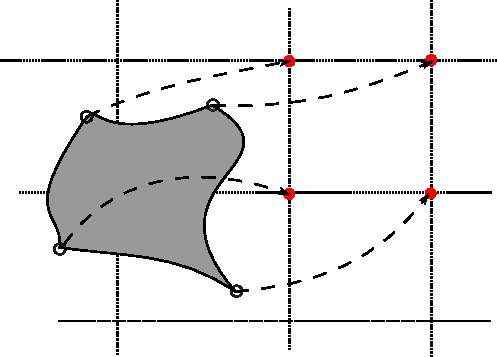
\includegraphics[width=0.5\linewidth]{semi_lagrangian2D.pdf}
  \caption{Illustration of a time-step in a forward semi-Lagrangian scheme.}
  \label{fig:semi-lagrang}
\end{figure}

The main advantage of semi-Lagrangian schemes is their weaker stability
criteria. According to \cite{Smolarkiewicz1992}, it can be written in 1D as:
\begin{equation}
  ||\frac{\partial v}{\partial x}|| \Delta t < 1
\end{equation}
and can be interpreted geometrically as the fact that trajectories do not cross.
This is less restrictive than the Courant-Friedlich-Lewy condition (CFL) generally
used for 1D Eulerian models:
\begin{equation}
  \max{( \frac{u \Delta t}{\Delta x} )} < 1.
\end{equation}
In practice, this gain in the time-step for grid-point semi-Lagrangian can be
used to improve the accuracy of the model (with a finer resolution or improved
parametrizations). \DIFdelbegin \DIFdel{This }\DIFdelend \DIFaddbegin \DIFadd{Another advantage is that backwards trajectories only need to
be computed once for multi-tracers advection. These advantages }\DIFaddend led to a wide
adoption for operational models (see Table~\ref{tab:sl-models} for a list of
examples). 
\begin{table}
  \centering
  \begin{tabular}{ll}
    \toprule
    Centre & Reference \\
    \midrule
    \gls{CMC} & \cite{Cote1998} \\
    \gls{ECMWF} & \cite{Ritchie1995}\\
    United Kingdom Meteorological Office & \cite{Davies2005} \\
    Danish Meteorological Institute & \cite{Nair2002} \\
    China Meteorological Association & \cite{Chen2008} \\
    Meteo-France & \cite{Bubnova1995} \\
    Hydrometcentre of Russia & \cite{Tolstykh2001} \\
    \gls{JMA} & \cite{JMA2013}\\
    \bottomrule
  \end{tabular}
  \caption{Operational models using semi-Lagrangian approaches}
  \label{tab:sl-models}
\end{table}
Yet, semi-Lagrangian do not preserve mass inherently. To address that issue,
mass fixers can be used to adjust the scheme such as mass is preserved globally.
Examples of this method are given in
\cite{Priestley1993,Moorthi1993,Williamson1994}. Another way is to use
cell-integrated methods which are conservative by nature, an approach explained
in Section~\ref{subsub:cisl}. Another disadvantage of the semi-Lagrangian
formulation is the interpolation step: not only is it expensive, but it
creates numerical diffusion. 

\subsection{Finite-volume schemes}
\label{subsec:fv_schemes}
Conservation properties and scalability are two current trends for the
next-generation climate and weather models. As such, spectral and
semi-Lagrangian methods are now being reconsidered: the former as they are not
easily scalable, the latter as they are not inherently conservative.  \DIFaddbegin \DIFadd{An
illustration of this trend can be found in~\mbox{%DIFAUXCMD
\cite{Kukkonen2012}
}%DIFAUXCMD
, where several
operational chemical weather forecasting models are compared for regional
simulations. In this comparison, the majority of the models are Eulerian. This
trend is confirmed by another comparison of atmospheric chemistry and climate
models in~\mbox{%DIFAUXCMD
\cite{Lamarque2013}
}%DIFAUXCMD
. The table~\ref{tab:accmip} resume the different
type of advection schemes.
}

\begin{table}
  \centering
  \caption{\DIFaddFL{Different advection schemes from the comparison in~\mbox{%DIFAUXCMD
\cite{Lamarque2013}
}%DIFAUXCMD
.}}
  \label{tab:accmip}
  \begin{tabular}{lcc}
    \toprule
    \DIFaddFL{Model }& \DIFaddFL{Advection scheme }\\
    \midrule 
    \DIFaddFL{CICERO-OsloCTM2 }& \DIFaddendFL Finite-volume \DIFaddbeginFL \\
    \DIFaddFL{CMAM  }& \DIFaddFL{Spectral }\\
    \DIFaddFL{EMAC }& \DIFaddFL{Semi-Lagrangian }\\
    \DIFaddFL{GEOSCCM }& \DIFaddFL{Finite-volume }\\
    \DIFaddFL{GISS-E2-R }& \DIFaddFL{Finite-volume  }\\
    \DIFaddFL{HadGEM2 }& \DIFaddFL{Semi-Lagrangian }\\
    \DIFaddFL{LMDzORINCA }& \DIFaddFL{Finite-volume  }\\
    \DIFaddFL{MIROC-CHEM }& \DIFaddFL{Semi-Lagrangian }\\
    \DIFaddFL{MOCAGE }& \DIFaddFL{Semi-Lagrangian }\\
    \DIFaddFL{NCAR-CAM }& \DIFaddFL{Finite-volume }\\
    \DIFaddFL{STOC-HadAM3 }& \DIFaddFL{Lagrangian }\\
    \DIFaddFL{UM-CAM }& \DIFaddFL{Finite-volume }\\
    \bottomrule
  \end{tabular}
\end{table}


\DIFadd{Finite-volume }\DIFaddend schemes are well-suited to solve conservation laws, \textit{i.e.},
the air and tracer continuity equations for CTMs. Finite-volume schemes are also
very useful for dynamical cores, which solve the conservation of total energy,
angular momentum and entropy.

Finite-volume schemes are derived by integrating the flux-form equations over a
control volume and in time. In the case of CTMs, the air or tracer mass is then
updated by the fluxes through the control volume during a time-step. Choosing a
proper control volume remains an open question but finite-volume schemes can be
adapted to a wide range of geometry. A review of most common grids for
atmospheric transport is presented in Section~\ref{sec:grids}.
Most of the current finite-volume schemes have an order equal or lower than
three. It is possible to use higher-order schemes such as WENO
(\cite{Jiang1999}) but they require a large number of cells, which will impact
scalability. It should also be noted that finite-volume schemes have a wide
range of application and the choices made for Pangolin are very specific to the
atmospheric transport. For a more general review, the reader can refer
to~\cite{LeVeque2002}.

Finite-volume schemes can fall into two categories: flux-form and
semi-Lagrangian. Flux-form schemes are based on the flux-form equation, in our
case Eq.\eqref{eqn:cont_flux}, while semi-Lagrangian schemes are based on the
Lagrangian form, shown in Eq.\eqref{eqn:cont_lagrang}. It can be shown that
these two formulations are equivalent (see~\cite{Machenhauer2009}). The
difference between the two stems from the approximations made for each approach,
such as the mass integral and the trajectories.

\subsubsection{Semi-Lagrangian }
\label{subsub:cisl}
While in ''traditional'' semi-Lagrangian methods, values are interpolated from
grid-points, the finite-volume version advects average values over the cell
area. The discretization of the equations leads to the following scheme: the
average value over the regular cell can be computed from the integrated value
over the irregular departure cell. So the main difficulty is to compute this
integrated value over the departure cell explicitly. These schemes are referred
to as \gls{DCISL}. 

To solve the 3D continuity equation, we can simplify the problem by considering
that horizontal and vertical advection are separated. This means that we use
vertically integrated variables and only focus on the horizontal advection. It
is also possible to consider a full 3D transport for semi-Lagrangian
finite-volume schemes but this increases the complexity, especially for
mass preservation. 2D schemes can be divided into two categories: fully 2D and
"cascade" schemes.

We first detail fully 2D schemes. To approximate the integral, the first step
is to define the geometry of the departure cell, which is difficult to compute
efficiently due to the spherical geometry. We present some solutions in 2D but
the extension to the spherical geometry is presented in~\cite{Machenhauer2009}.
In 2D, one solution is to find the four departure points from the trajectories%
\footnote{The trajectories can be computed either starting from the
Eulerian grid ("backward") or to the Eulerian grid ("forward") and a common
trajectory algorithm is the one presented by~\cite{Staniforth1991}.}%
and link them with straight lines to
create a polygon (see~\cite{Rancic1992}). Another possibility is to use
quadrilaterals with sides parallel to the x- and y-axis as in~\cite{Nair2002}.
The second step is to reconstruct the distribution of the transported variable
in this new Lagrangian cell. Common reconstructions use constant, first-order or
even higher-order polynomials.

Another approach is to use a "cascade" scheme which splits the 2D integral into
two 1D integrals. For that, an intermediate grid must be constructed. The
algorithm is as follows: first, the integral is computed from the Eulerian cells
to the intermediate grid. Then the second integral is computed from the
intermediate grid to the Lagrangian cells. More details and illustrations about
this scheme can be found in~\cite{Purser1991}. Cascade schemes have this
advantage that they can be easily extended to the 3D case.

\subsubsection{Flux-form}
Another finite-volume approach, similar in the result but different in the
method, is to consider that the mass is modified according to the fluxes passing
through the walls of cells. As for \gls{DCISL} schemes, there are full 2D
schemes as well as operator-splitting schemes, where 1D operators are applied
successively. Furthermore, flux-form schemes can easily be extended to 3D using
operator splitting than their semi-Lagrangian counterpart. We present in more
details this approach in the next section.

\section{Flux-form finite-volume schemes}
\label{sec:fv_schemes}
Here, we focus on solving the equations \eqref{eqn:air} and \eqref{eqn:tracer}
using flux-form finite-volume schemes. The first equation describes the
conservation of "moist air", that is, atmospheric air with all of its chemical
components. The second equation describes the conservation of a tracer, defined
by the ratio of the tracer mass over the air mass in a given volume. The
accuracy of moist air is especially important in meteorology as the flow of air
mass determines pressure and weather dynamics. Furthermore, the conservation of
linear relations between chemical tracers is especially important for
\gls{CTM}s.

To derive the flux-form version, we consider 2D Eulerian cells without making
assumptions on their shape. The cell area is noted $\mathcal{A}$ and its
boundary $\partial \mathcal{A}$. First, we integrate both the continuity and
tracer conservations~\eqref{eqn:air} and~\eqref{eqn:tracer} over a cell grid:
\begin{align}
  \frac{\partial m}{\partial t}=\frac{\partial}{\partial t} {\int_{\mathcal{A}}
\rho}
&= \int_{\partial \mathcal{A}} (\rho {\bf V}\cdot{\bf n} \;\mathrm{d}S),
\label{eqn:air2}\\
\frac{\partial mq}{\partial t}=\frac{\partial}{\partial t} {\int_{\mathcal{A}}
\rho q} &= \int_{\partial \mathcal{A}} (\rho q {\bf V}\cdot {\bf n} \;\mathrm{d}S).
\label{eqn:tracer2}
\end{align}
Then, integrating over a time-step yields:
\begin{align}
[m]^{n+1} &= [ m]^{n} + \int_{t_n}^{t_{n+1}}
\Big( \int_{\partial \mathcal{A}} \rho {\bf V}\cdot{\bf n}\;\mathrm{d}S \Big) \mathrm{d}t,
\label{eqn:mintegral} \\
[ mq]^{n+1} &= [ mq]^{n} + \int_{t_n}^{t_{n+1}}
\Big( \int_{\partial \mathcal{A}} \rho q {\bf V}\cdot{\bf n}\;\mathrm{d}S \Big) \mathrm{d}t,
\label{eqn:qintegral}
   \end{align}
where $[m]^{n+1}$ is the average air mass in the considered cell at time $t_n$
and $[mq]^{n+1}$ the average tracer mass at the same time.
At this point, no hypothesis were made about the shape of the cells.
As an illustration, we consider the 1D version of these equations on a regular
latitude-longitude grid. If we consider the $i$-th cell, with its borders noted
$i-1/2$ and $i+1/2$, we have:
\begin{align}
  \label{eqn:air_update}
  {m}_i^{n+1} &= m_i^{n} + U_{i-1/2} - U_{i+1/2},\\
  \label{eqn:tracer_update}
  [{m_iq_i}]^{n+1} &= [m_iq_i]^{n} + F_{i-1/2} - F_{i+1/2},
\end{align}
where $U_{i-1/2}$ is the flux of air mass passing through the cell wall $i-1/2$ and
$F_{i-1/2}$ is the flux of tracer mass passing through the same cell wall.
However, it should be noted that other geometries are possible and flux-form can
be used in a variety of grids. In particular, Section~\ref{subsec:2d_ff} explains how it was
adapted to our non-regular grid.

The accuracy of the scheme depends on the accuracy of the fluxes computation,
namely $U$ and $F$. While the air mass fluxes $U$ can be computed easily knowing
the winds and the size of the cell borders, there is no exact formula for $F$ as
we only have discretized data at our disposal.  It is then approximated as the
mean ratio $\hat{q}$ value passing through the cell border times the air mass
flux: $F=\hat{q}\,U$. Therefore, we have to reconstruct the tracer mass
distribution in the cell to be able to integrate it. Different reconstruction
are highlighted below in the 1D case. The extension to 2D is detailed in
Section~\ref{subsec:2d_ff}.

\subsection{Sub-grid distributions}
\subsubsection{First-order}
To reconstruct the mass distribution, polynomials are the more common
representation used in practice. The first proposal was made by
\cite{Godunov1961} where the distribution in each cell is reconstructed as a
constant function. It is a very simple requirement to preserve the
shape of the distribution but it is also very diffusive. To improve on that, the use
of a first-order polynomial was proposed by~\cite{Leer1977}. As the
reconstruction is locally linear for each cell, there is no continuity between
the cells.  Computing the slope can be done for example with
finite-differences (scheme I in~\cite{Leer1977}) or with a least-square fit
(scheme III in~\cite{Leer1977}, also called "slopes scheme" in the \gls{GCM}
community). The idea for Godunov's scheme and the two van Leer's schemes is
highlighted on Fig.~\ref{fig:godunov},~\ref{fig:vanleerI}
and~\ref{fig:vanleerIII} respectively.
\begin{figure}
  \subbottom[Godunov's method.]{%
    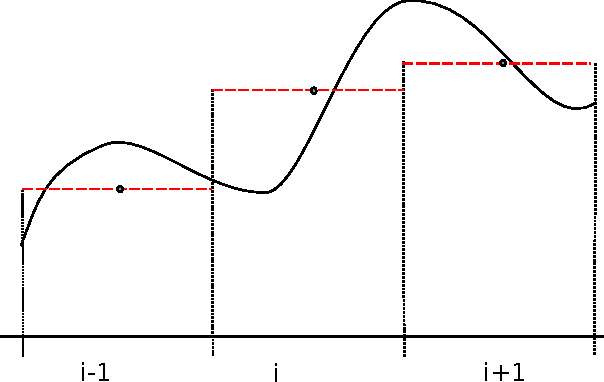
\includegraphics[width=0.48\linewidth]{godunov.pdf}
    \label{fig:godunov}}
  \hfill
  \subbottom[van Leer's scheme I: the slope is simply computed by finite
  differences.]{%
    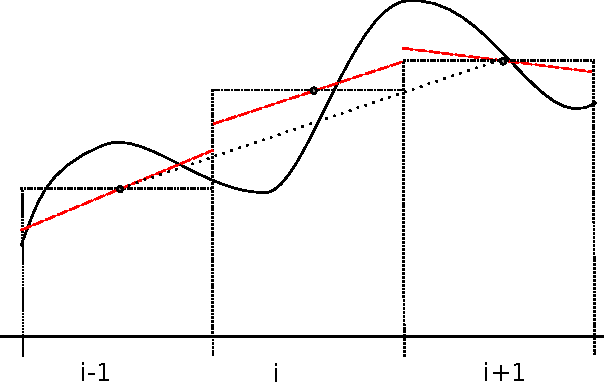
\includegraphics[width=0.48\linewidth]{vanleerI.pdf}
    \label{fig:vanleerI}}
  \caption{Constant and first-order reconstruction of the grid distribution
    (dark line). Cell average are shown as dotted lines and the reconstruction is
  the dashed red line.}
\end{figure}

\begin{figure}
  \subbottom[Van Leer's scheme III: the slope is computed with a least square
  method.]{%
    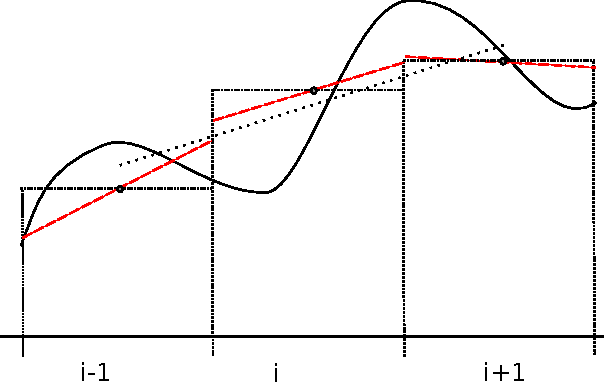
\includegraphics[width=0.48\linewidth]{vanleerIII.pdf}
    \label{fig:vanleerIII}}
  \hfill
  \subbottom[PPM: the reconstruction is smooth and uses the west and east value
  in the cell (shown as dots).]{
    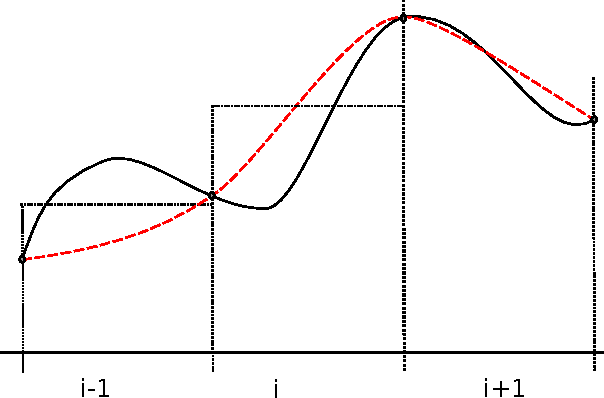
\includegraphics[width=0.48\linewidth]{ppm.pdf}
    \label{fig:ppm}}
  \caption{First and second-order reconstruction of the grid distribution (dark
    line). Cell average are shown as dotted lines and the reconstruction is the
  dashed red line.}
\end{figure}

The scheme was subsequently improved in~\cite{Leer1979}, who proposed a
monotonicity algorithm to reduce numerical oscillations. The slope is limited to
prevent that the new distribution in a cell does not exceed the mean value of the
adjacent cells. This is illustrated in Fig.~\ref{fig:slope_limit}.

\subsubsection{PPM and Prather}
It is also possible to use quadratic polynomials to reconstruct the mass
distribution, as shown by~\cite{Leer1977} (scheme V in the original paper). Van
Leer only used finite differences to evaluate the coefficients of the polynomial
but this led to the \gls{PPM}. A first version, proposed
by~\cite{Laprise1995}, defined the coefficients of the parabola by enforcing
mass preservation in the current cell and its two neighbours.  A second version
was proposed by~\cite{Colella1984}, where the west and east cell values are used
as initial conditions. This allows the reconstructed distribution to be
continuous across cell borders and the result is shown in
Fig.~\ref{fig:ppm}. Polynomials are only one choice among many, as long as the
chosen function can preserve mass. For example, \cite{Xiao2002} used rational
functions and~\cite{Zerroukat2002} used parabolic splines.

To ensure monotonicity, a simple filter was proposed by~\cite{Colella1984}.
Other filters exist, for example in~\cite{Lin1996}, the filter was modified as
to prevent undershooting only. An example for more advanced filters can be found
in~\cite{Zerroukat2005}, which aims at preventing the clipping of peaks while
removing grid-scale noise anyway.  The PPM scheme can be extended to 2D, as
shown by~\cite{Rancic1992} but is quite expensive from a computational point of
view. Furthermore, using 1D filters in this case does not remove all negative
values so additional filters are needed.

Another well-known second-order reconstruction is the \gls{SOM} scheme
introduced by~\cite{Prather1986}. The reconstruction is written as:
\begin{align*}
  f(x,y,z) = a_0 &+ a_1 K_x(x) + a_2 K_y(y) + a_3 K_z(z)\\
  & + a_4 K_{xx}(x) + a_5 K_{yy}(y) + a_6 K_{zz}(z)\\
  & + a_7 K_{xy}(x,y) + a_8 K_{xz}(x,z) + a_9 K_{yz}(y,z),
\end{align*}
where the $K$ are polynomial orthogonal functions. In particular, $K_x$ is a
first-order polynomial in $x$, $K_{xx}$ second-order and $K_{xy}$ a first-order
in $x$ and $y$. This scheme is more accurate compared to the previous schemes
and it preserves second-order moments (the 6 coefficients $a_i$ with $i=4..9$.).
However, it is also more computationally expensive and needs to store 10 tracers
(the $a_i$, $i=1..10$).

\subsection{2D flux-form schemes}
\label{subsec:2d_ff}
The simplest approach to extend the 1D schemes mentioned previously to the 2D
case is to simply combine the two 1D operators simultaneously. For simplicity,
we note $Q^n=[mq]^n$ the tracer mass at the time-step $n$. The update of tracer
mass during one time-step is then:
\begin{equation}
  Q^{n+1} = Q^{n} + H_{zonal}(Q^n) + H_{merid}(Q^n),
\end{equation}
where $H_{zonal}$ (resp. $H_{merid}$) is the 1D operator corresponding to the
zonal (resp. meridional) advection.  This approach is stable for 1D
reconstruction as shown by~\cite{Leonard1996} but not for the 2D
reconstruction. Therefore, we have to apply each operator sequentially:
\begin{align}
  \label{eqn:split1}
  &\widehat{Q}_{zonal} = Q^{n} + H_{zonal}(Q^n),\\
  \label{eqn:split2}
  &Q^{n+1} = \widehat{Q}_{zonal} + H_{merid}(\widehat{Q}_{zonal}).
\end{align}
Unfortunately, this approach introduces a directional bias due to its
non-symmetrical nature. A simple way to avoid that is to alternate the operators
at each time-step, also called operator-splitting. For example, the first
time-step will use $H_{zonal}$ then $H_{merid}$ while the next will apply
$H_{merid}$ then $H_{zonal}$. Another solution is to define a symmetric scheme:
\begin{equation}
  Q^{n+1} = Q^n + H_{zonal}\Big(\frac{Q^n + \widehat{Q}_{merid}}{2}\Big) + 
  H_{merid}\Big(\frac{Q^n + \widehat{Q}_{zonal}}{2}\Big).
\end{equation}
Yet, all these schemes introduce a splitting error: a spatially uniform field with
divergence-free winds will not be preserved, as the field will be deformed in
one direction by the scheme. \cite{Lin1996} proposed an algorithm to address
that issue by compensating the error due to the deformation.

Operator-splitting approaches are computationally efficient and easy to extend
to several dimensions. But if we examine them from a semi-Lagrangian
point-of-view, we cannot integrate on the exact departure area exactly due to an
inconsistency due to the splitting. To try to solve that issue, the use of fully
2D fluxes was studied (see for example~\cite{Rasch1994,Dukowicz2000}). But the
fluxes in the cross-directions must be written explicitly, contrary to the
operator-splitting approach, where there are "automatically" accounted for. It
is also a more expensive approach.

\subsection{Scheme chosen in Pangolin}
In Pangolin, our goal is not to invent a new scheme, but rather implement an
already-existing but efficient scheme on our custom grid (presented in
Section~\ref{subsec:pango_grid}). The most important requirements for our
scheme is its flexibility to adapt to our non-regular grid, mass preservation
and scalability on parallel computers. We have chosen a flux-form finite-volume
approach as it preserves tracer mass globally and locally. It is also
considerably easier to parallelize than the semi-Lagrangian alternative.  The
parallelization issue is then reduced to a domain decomposition problem detailed
in Section~\ref{subsec:domain_decompos}.

The current version of Pangolin is bi-dimensional but a future version should
deal with 3D advection. The operator-splitting approach was chosen for
simplicity reasons. Among the different flux-form schemes, the Van Leer scheme I
was chosen. While it may be less accurate than higher-order schemes such as
\gls{PPM}, higher-order reconstruction increases data volume in a
parallelization based on a message-passing approach (see
Section~\ref{sec:strategy}). We strive to reduce communications, so a first-order
reconstruction in each direction is a good compromise. On top of that, in an
operator-splitting algorithm, the formal order cannot be greater than 2.  As
shown in the test results of Section~\ref{sec:comparison}, we aim at
achieving the same accuracy than higher-order schemes with finer resolutions.
Finally, it should be remembered that Pangolin is essentially a parallel framework
using a custom quasi area-preserving grid, on which several schemes can be
plugged. The results showed here are obtained from a given transport scheme but
this scheme can be replaced according to the needs of the modellers.

We now summarize the different steps of the scheme. The equations to solve are
Eq.~\DIFdelbegin %DIFDELCMD < \eqref{eqn:air} %%%
\DIFdelend \DIFaddbegin \eqref{eqn:air2} \DIFaddend and Eq.~\DIFdelbegin %DIFDELCMD < \eqref{eqn:tracer}%%%
\DIFdelend \DIFaddbegin \eqref{eqn:tracer2}\DIFaddend . In 1D, they are discretized to
arrive to the form presented in Eq.~\eqref{eqn:air_update}
and~\eqref{eqn:tracer_update}. Eq.~\eqref{eqn:tracer_update} can be omitted for
non-divergent flows since the divergence of the mass fluxes is null and the
mass inside a cell is constant: $[m]^{n+1} = [m]^{n}$. \\
To compute the fluxes $f_{i+1/2}$, we have to find the mean value
$\widehat{q}_{i+1/2}$, given by the van Leer~I scheme:
\begin{align}
 \widehat{q}_{i+1/2} =
  \begin{cases}
    q_i + \left(1 -  \frac{u_{i+1/2} \Delta t}{\Delta x}\right)(\delta q)_i
    \quad &\text{if} \quad u_{i+1/2} > 0,\\
    q_{i+1} - \left(1 + \frac{u_{i+1/2} \Delta t}{\Delta x}\right) (\delta q)_{i+1}
    \quad &\text{otherwise},
  \end{cases}
  \label{eqn:vanleer1}
\end{align}
\begin{figure}
  \centering
  \subbottom[Positive winds]{%
    \includegraphics[width=0.3\linewidth]{vanleer1.pdf}
  }
  \subbottom[Negative winds]{%
    \includegraphics[width=0.3\linewidth]{vanleer2.pdf}
  }
  \caption{van Leer scheme for positive and negative winds. The
  distribution of the tracer is shown as broken lines. The grey area is the
  quantity of tracer passing through the interface during a~time-step.}
\label{fig:van_leer}
\end{figure}
This reconstruction is illustrated on Fig.~\ref{fig:van_leer}, where the broken
lines represent the tracer distribution for cells $i$ and $i+1$. Depending on
the wind direction, the tracer mass passing through the interface $i+1/2$ either
comes from cell $i$ when $u_{i+1/2} > 0$ or $i+1$, when $u_{i+1/2} < 0$. 
Computing the slope can be done with finite-difference :
  $(\delta q)_i = \frac{1}{2} (q_{i+1}-q_{i-1})$.
We use in practice the slope limiter of~\cite{Leer1979}:
\begin{align}
  (\delta q)_i =
  \min\big(\frac{1}{2} |q_{i+1}-q_{i-1}|, 2|q_{i+1}-q_i|, 2|q_i-q_{i-1}|\big)
  \times \text{sign}(q_{i+1} - q_i),
  \label{eqn:slope}
\end{align}
if $q_i$ lies in between $q_{i-1}$ and $q_{i+1}$, and $(\delta q)_i =0$
otherwise. An example of the limiter is shown on fig.~\ref{fig:slope_limit}.
\begin{figure}
  \subbottom[The limiter ensures the value is cell $i$ is not greater than the
  average of its two neighbours (dotted line).]{%
    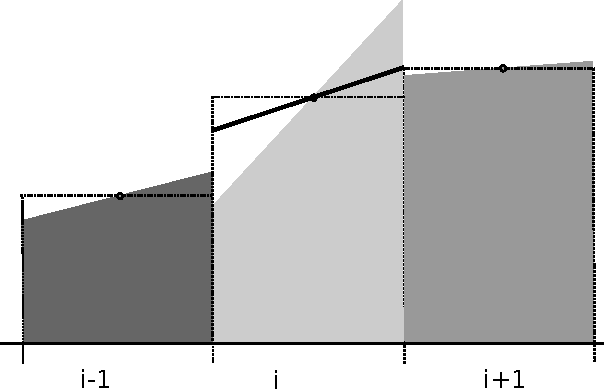
\includegraphics[width=0.4\linewidth]{vanleer_limiter.pdf}
  }
  \hfill
  \subbottom[The slope in cell $i$ is set to $0$ as the cell average is a local
  maximum.]{%
    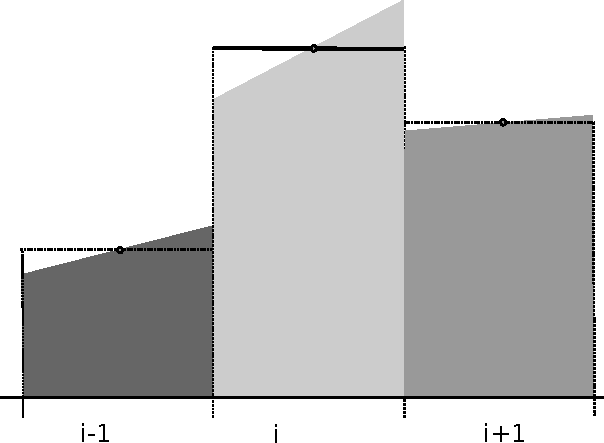
\includegraphics[width=0.4\linewidth]{vanleer_limiter2.pdf}
  }
  \caption{van Leer's slope limiter in the 1D case. The limited slope is shown
  as a dark line, while the reconstruction is shown as broken lines.}
  \label{fig:slope_limit}
\end{figure}

To extend the 1D algorithm to 2D, we use the simplest operator-splitting algorithm:
first, the tracer and air mass are advected in the zonal direction, then in the meridional
direction as in Eq.~\eqref{eqn:split1}
and~\eqref{eqn:split2}.

\section{Choosing a grid}
\label{sec:grids}
\subsection{Introduction}
There are several ways of gridding the sphere and it is still an active topic of
research. In general, the choice of the grid impacts the discretization and the
scheme. More precisely, it can impact key properties of the scheme such as mass
conservation or accuracy.  In some cases, the grid structure can even generate
noise. On top of that, the sphere presents unique challenges: finding an uniform
resolution without singularities or clustering is not trivial. The grid also
impacts computational efficiency and scalability on parallel architectures.

\begin{figure}
  \begin{minipage}{0.48\linewidth}
    \centering
    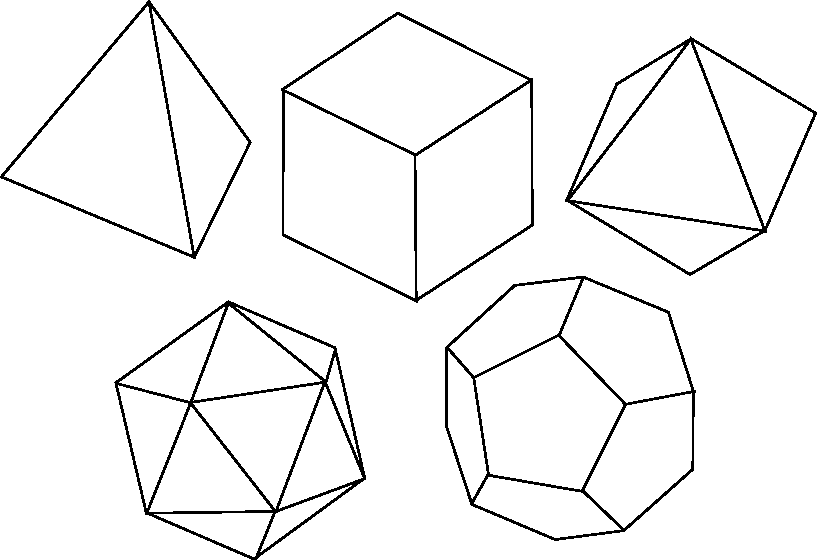
\includegraphics[width=\linewidth]{platonic.pdf}
    \caption{The five platonic solids. From left to right and top to bottom:
      tetrahedron, cube, octahedron, dodecahedron, icosahedron.}
    \label{fig:platonic}
  \end{minipage}
  \hfill
  \begin{minipage}{0.48\linewidth}
    \centering
    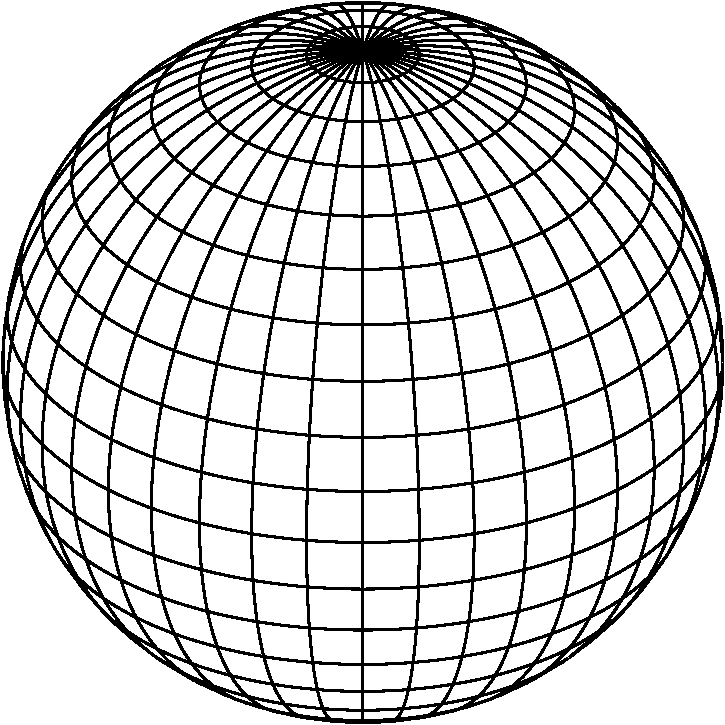
\includegraphics[width=0.8\linewidth]{latlon.pdf}
    \caption{Regular latitude-longitude grid with 20 latitudes.}
    \label{fig:latlon}
  \end{minipage}
\end{figure}
It can be shown there are only five ways to tile the sphere uniformly. For that,
we have to use one of the five platonic solids (shown in
Fig.~\ref{fig:platonic}) and do a \gls{gnomonic} of each face onto the sphere.
However, the resulting grids would be too coarse as platonic solids have at most
20 faces. This leads us to make compromise to tile the sphere: we cannot have
uniformity and orthogonality and to be free of singularities. Singularities are
not necessarily a drawback but some grids, especially the regular
latitude-longitude grid, have cell clustering near these singularities. Then
CFL conditions in Eulerian formulations imply poor scaling when the resolution
increases. For that reason, uniform or quasi-uniform grids are preferred.
Orthogonality is another interesting property but is less important for
\gls{CTM} than for dynamical cores (see~\cite{Staniforth2012} for more
information about this and other impacts of grids on dynamical cores). Yet, it
helps making neighbour computation and thus flux computation easier in our case.
Another possible constraint is the geometry of the cells. Quadrilaterals are the
most common cells in practice but some grids can use more "exotic" shape, which
can restrict the choice of the scheme.

Here, we highlight different categories of grids with their pros and cons, while
the grids themselves are explained in more details in Section~\ref{subsec:grids}.
We can generate orthogonal quadrilateral grids with a \gls{conformal} projection
but it implies singularities on the sphere and some resolution clustering.
Regular latitude-longitude and conformally projected cubic grids are two
examples of that. Singularities can be avoided with composite grids
while achieving quasi-uniformity. The downside is the increased cost of the
overlapped regions. Overlaps also impact scalability significantly due to the
increase communication in these regions. It is also not easy to preserve mass
accurately and efficiently on the overlapped region. If we give up on
orthogonality, we can avoid both clustering and overlaps and still use
quadrilaterals. The gnomonically projected cubic grid is one example of that.
Other approaches use an orthogonal dual (for example, by dividing the
quadrilaterals into "kite"-shaped polygons). If we give up quadrilaterals, we
can manage the quasi-uniformity and have an orthogonal dual with icosahedral
grids.

\subsection{Review}
\label{subsec:grids}
\subsubsection{Latitude-longitude}
This grid is the most popular as it has a rectangular structure, is orthogonal
and is very natural to use. However, the convergence of meridians at the poles
(see Fig.~\ref{fig:latlon}) is an important problem. It imposes a severe
constraint on the time-step in Eulerian formulations. The resolution
is anisotropic so there is a decrease in computation efficiency. It also leads
to poor scaling concerning communications around the poles. To deal with the
time-step constraint, this grid is now often used with semi-Lagrangian
approaches, which are less sensible to stability requirements. As an
illustration, the \gls{NCAR} in their CAM3 model implemented a flux-form
semi-Lagrangian model. An improvement of the latitude-longitude grid was
proposed by~\cite{Kurihara1965}, where the number of cells at a latitude
decreases as the latitude gets closer to the pole (see
Section~\ref{subsec:pango_grid}).

\subsubsection{Cubed-sphere grids}
Cubed-sphere grids can fall into two categories. The first uses the
\gls{gnomonic} projection and was proposed by~\cite{Sadourny1972}: Cartesian
coordinates are used on each face of the cube and then projected gnomonically.
This approach used finite-differences and did not enjoy much popularity at the
time but it generated renewed interest with~\cite{Rancic1996}
or~\cite{Harris2011}.
The equi-distant version of this grid uses an uniform Cartesian grid on each
face, leading to a non-uniform grid once projected. The equi-angular version of
this grid does the inverse: uniformly spaced meridians are projected, resulting
into an non-uniform Cartesian grid. An illustration is shown in
Fig.~\ref{fig:gnomonic_cubic}

\begin{figure}
  \begin{minipage}{0.48\linewidth}
    \centering
    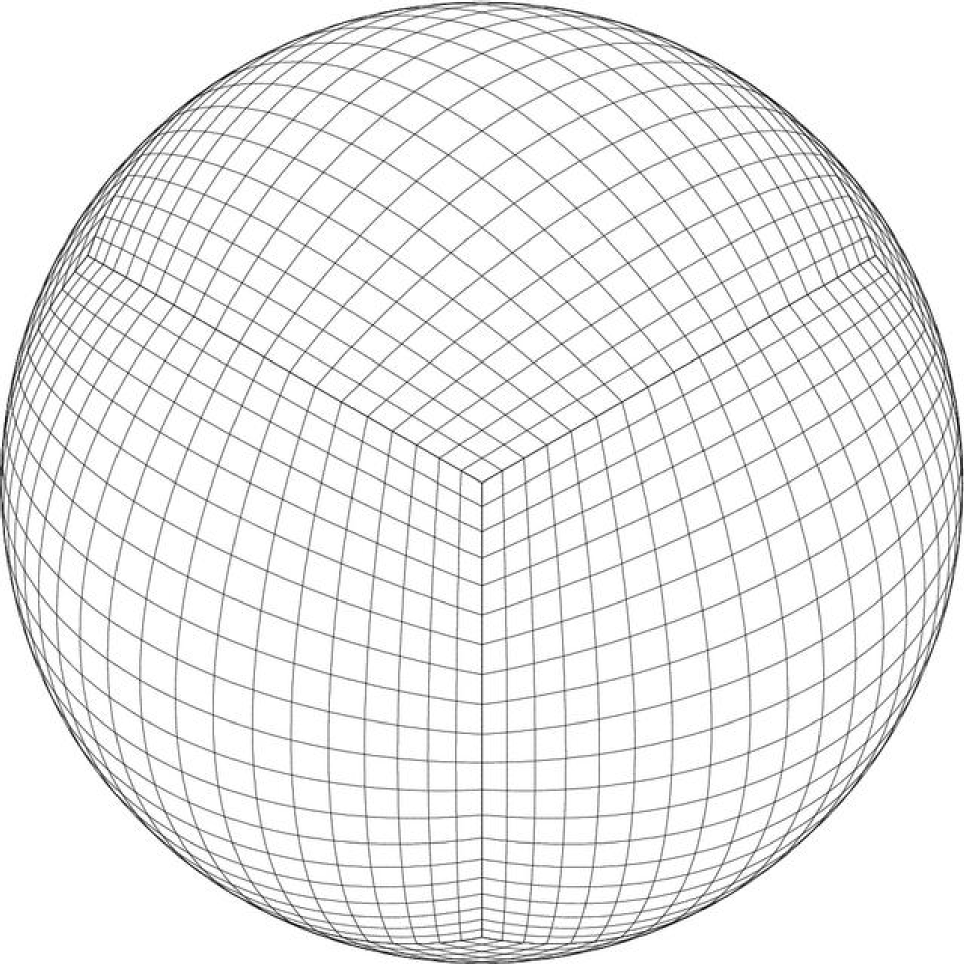
\includegraphics[width=\linewidth]{gnomonic_cubic.png}
    \caption{Equi-distant gnomonically projected grid (from~\cite{Putman2007}).}
    \label{fig:gnomonic_cubic}
  \end{minipage}
  \hfill
  \begin{minipage}{0.48\linewidth}
    \centering
    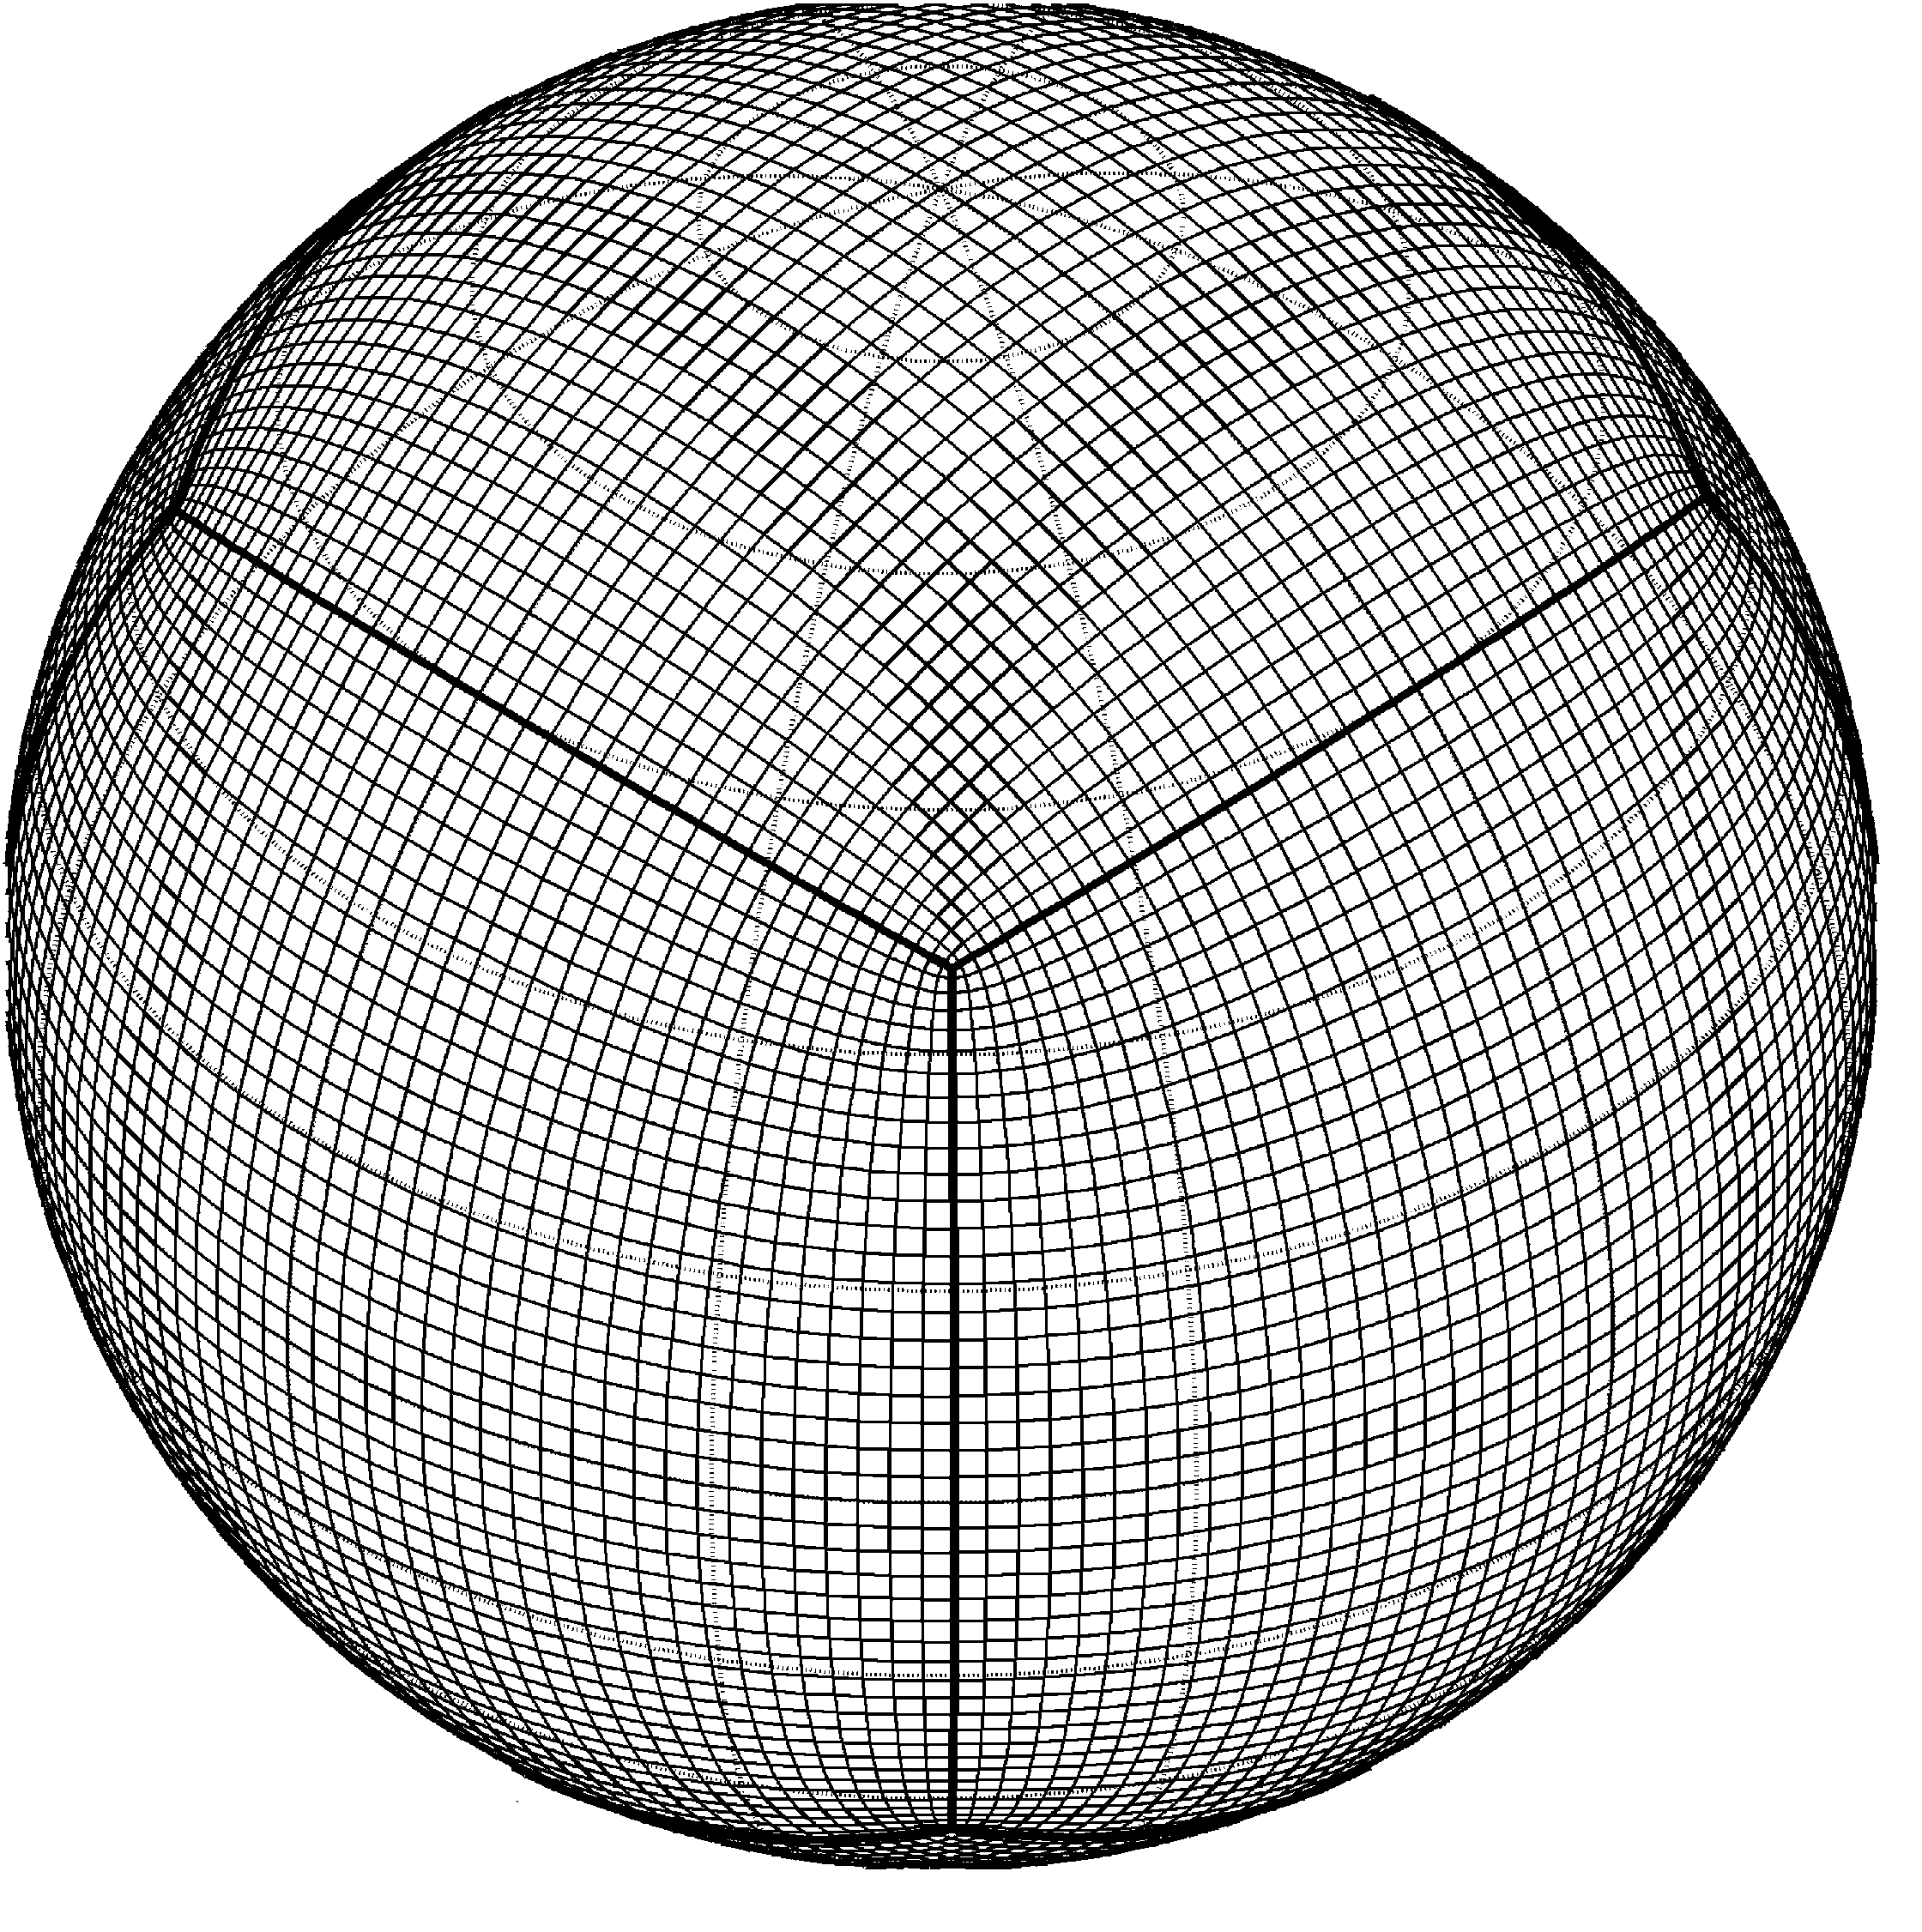
\includegraphics[width=\linewidth]{conformal_cubic.png}
    \caption{Equi-distant conformally projected grid (from~\cite{Putman2007}).}
    \label{fig:conformal_cubic}
  \end{minipage}
\end{figure}
The ratio of the maximum grid length over the minimum is 5.2 for the
equi-distant version and 1.3 for the equi-angular version. As a reference, this
can be compared to the composite grid of~\cite{Phillips1962} which claims a
ratio of 1.2 (see below).  Each face of the grid is free of singularities but
is not orthogonal. On the sphere, the eight vertices of the cube are still
singularities though.  If the uniformity requirement is relaxed, some
orthogonality can be gained. The balance was studied by~\cite{Putman2007}.
If a \gls{conformal} projection is used, each face is free of singularities and
also preserves orthogonality. Yet the eight vertices of the cube are still
singularities and resolution clustering can be seen around them as shown on
Fig.~\ref{fig:conformal_cubic}.

\subsubsection{Composite grids}
 One way to avoid singularities is to "patch" several, partially overlapping,
grids to create a composite (or overset) grid.
\cite{Phillips1957} proposed a grid separated into a tropical belt and two
square polar \gls{stereographic} grids. The ratio maximal/minimal grid length is then
1.373 but can be reduced to~1.2. This grid was improved by~\cite{Browning1989}
by removing the tropical belt, leading to two overlapping \gls{stereographic}
coordinates, one on each hemisphere. This is illustrated on
Fig.~\ref{fig:composite_grid}.
In this configuration, the previous ratio is then increased to 2.

\begin{figure}
  \begin{minipage}{0.48\linewidth}
    \centering
    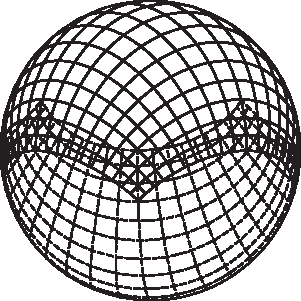
\includegraphics[width=\linewidth]{two-patches.pdf}
    \caption{Two-patch grid with stereographic coordinates for each patch (taken
      from~\cite{Williamson2007}).}
    \label{fig:composite_grid}
  \end{minipage}
  \hfill
  \begin{minipage}{0.48\linewidth}
    \centering
    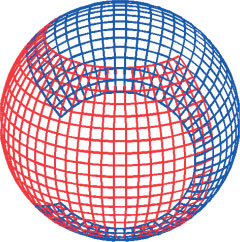
\includegraphics[width=\linewidth]{yin-yang.jpg}
    \caption{Yin-Yang grid (taken from~\cite{Williamson2007}).}
    \label{fig:yin-yang}
  \end{minipage}
\end{figure}

Another composite grid is the Yin-Yang grid introduced by~\cite{Kageyama2004},
which consists of two latitude-longitude grids "sewn" together (see
Fig.~\ref{fig:yin-yang}) and normal to each-other.
This grid is quasi-uniform without singular points but possesses an overlapping
region for which interpolation is needed. Global mass conservation can be
achieved using the algorithm presented in~\cite{Peng2006} which ensures the
fluxes at the boundary are identical on each "patch". The Yin-Yang grid is
almost as efficient as the grid of~\cite{Phillips1957} but is easier to use in
practice. As an example of a practical application, a forecasting model using
the Yin-Yang grid is being developed at the \gls{CMC}
(see~\cite{Qaddouri2011}).

\subsubsection{Icosahedral grid}
Icosahedral grids are part of a larger set of grids called geodesic. The idea is
to approximate the surface of the Earth by refining a polyhedron. In practice, a
icosahedron is the most common choice, thus leading to icosahedral grids. The
\gls{DWD} uses this kind of grid, as shown in~\cite{Majewski2002}. There are
different ways to generate the grid for a given resolution. The easiest way is
to start with the icosahedron and subdivides each triangle until the desired
resolution is achieved. \cite{Tomita2001} proposed a way to improve the grid
using spring dynamics. By default, the grid points do not correspond to the
center of gravity of the corresponding control volumes. They suggested to link the
grid points with springs in order to place them at the equilibrium. Their approach
helps to reduce the noise due to numerical integration.

However, it seems harder to use high-order finite-difference approximations on
this grid, as well as for finite-volume schemes. \cite{Giraldo2000} 
proposed a Lagrange-Galerkin finite element approach to solve the issue.
Another related grid is the hexahedral grid used in the spectral element
dynamical core of~\cite{Giraldo2003}. The grid is generated by subdividing each
face of an hexahedron (polyhedra with six faces) into quadrilaterals with the
desired resolution and project them on the sphere.

\subsubsection{Other grids}
The Fibonacci grid is one example of the more exotic grids and was developed
by~\cite{Swinbank2006}. Its advantages are its uniformity and isotropy. An
illustration is shown on Fig.~\ref{fig:fibonacci}.
The grid is constructed with a Delaunay triangulation using the grid points.
When examining the dual mesh, most of the cells are irregular hexagons but there
are some pentagons and heptagons as well. The grid itself possesses analytical
features which are exploited to reduce the memory footprint and improve
scalability.

\section{Pangolin grid}
\label{subsec:pango_grid}
Our motivation for the model is to solve the "pole issue" mentioned previously
in an Eulerian context as we focus on flux-form finite-volume approaches. For
that, we have chosen to use a custom reduced grid. Orthogonality is lost and
the poles are two singularities but we achieve a rectangular structure and have
quasi-uniformity.

\subsection{Reduced grids}
Reduced latitude-longitude grids were examined in order to solve the clustering
around the poles in the regular latitude-longitude grids. The idea is to
decrease the number of cells as the latitudes get closer to the pole to
have an uniform grid. The first reduced grid was proposed by~\cite{Kurihara1965}
for finite-difference schemes, on which the number of cells at colatitude $i$ is
$4(i-1)$ (see Fig.~\ref{fig:kurihara}). Cell width (or longitudinal spacing) is
constant for a given colatitude and the cell height (or latitudinal spacing) is
also constant. \cite{Rasch1994} proposed a different approach: starting from the
Equator, we go towards the pole. If cells are "too close" to each other, there
are merged two by two. The criteria for the merge in the paper is the distance
between two consecutive cells should be less than $2/3$ of the distance at the
Equator. This can also be seen as a composite grid and is illustrated on
Fig.~\ref{fig:rasch}.

\defcitealias{ECMWF2004}{the ECMWF grids}
Gaussian grids are one example of grids where the latitudinal spacing is not
constant but uses the Gaussian quadrature instead. A Gaussian reduced grid was
proposed by~\cite{Hortal1990} for spectral methods. An illustration of the
"fully" reduced grid is shown in Fig.~\ref{fig:hortal}.  It should be noted that
the grid used in practice is quite similar to the reduced version
in~\cite{Hortal1990} but with a different number of cells nevertheless (see for
example~\citetalias{ECMWF2004}). 
\begin{figure}
  \begin{minipage}[b]{0.48\linewidth}
    \centering
    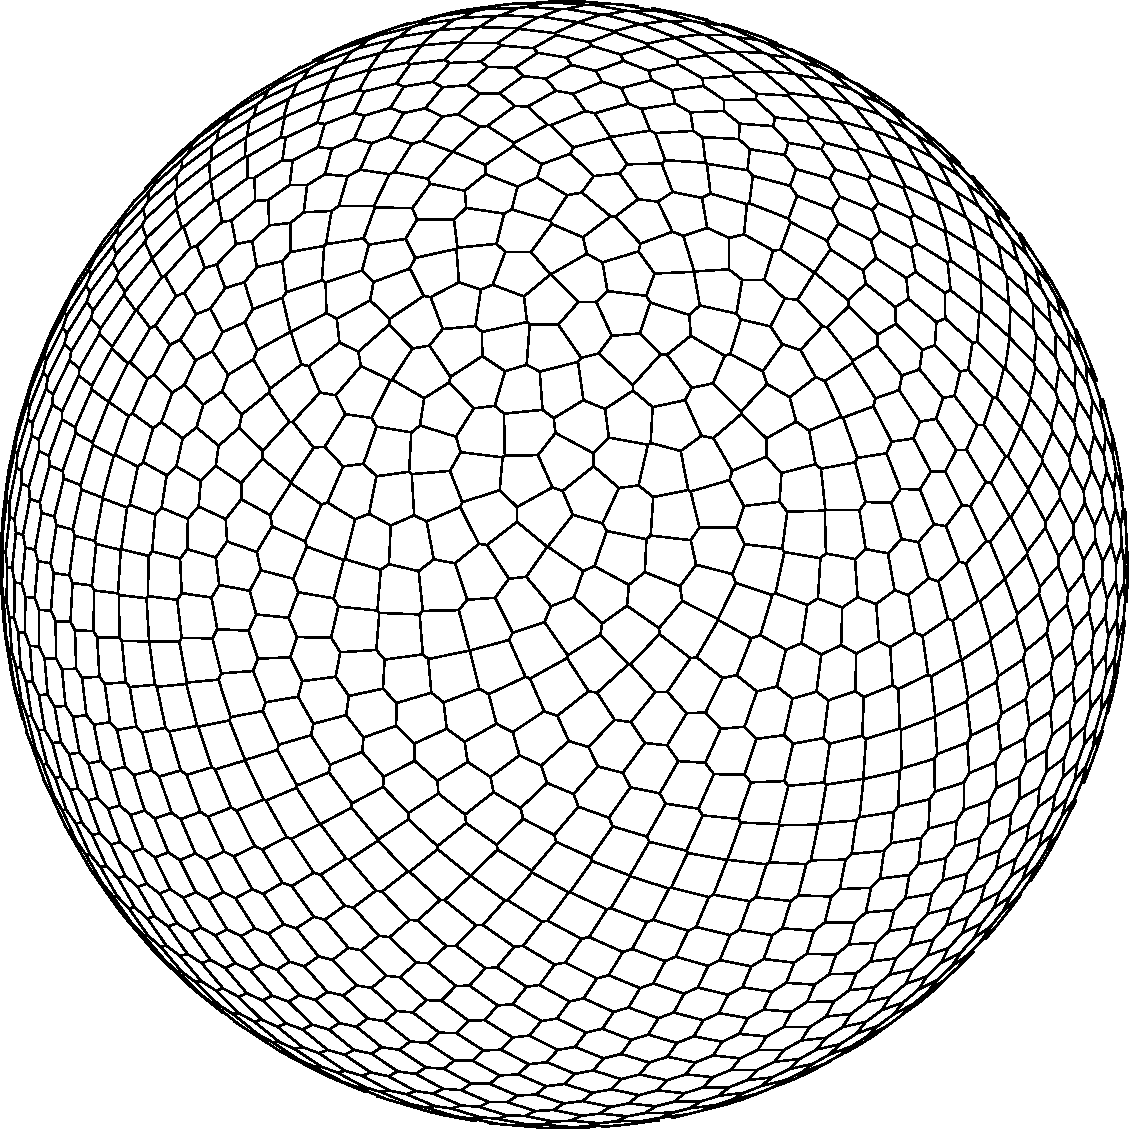
\includegraphics[width=\linewidth]{fibonacci.pdf}
    \caption{Fibonacci grid (from~\cite{Swinbank2006}).}
    \label{fig:fibonacci}
  \end{minipage}
  \hfill
  \begin{minipage}[b]{0.45\linewidth}
    \centering
    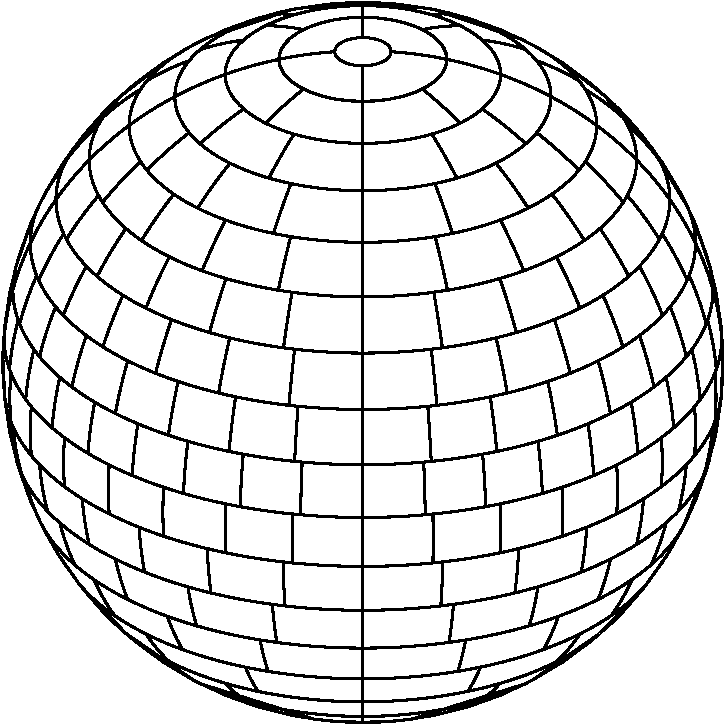
\includegraphics[width=\linewidth]{kurihara.pdf}
    \caption{Reduced grid by~\cite{Kurihara1965} with 20 latitudes (reconstructed).}
    \label{fig:kurihara}
  \end{minipage}
\end{figure}
\begin{figure}
  \begin{minipage}[t]{0.45\linewidth}
    \centering
    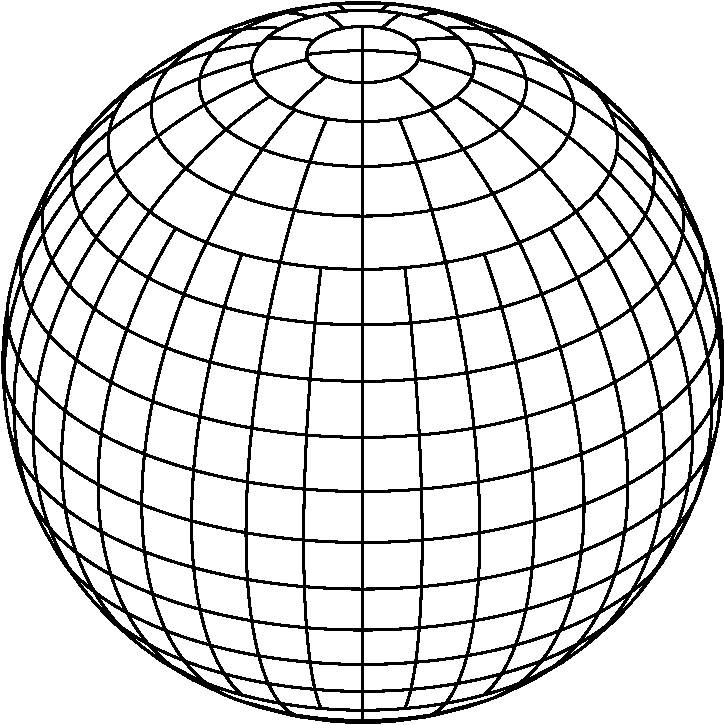
\includegraphics[width=\linewidth]{rasch.pdf}
    \caption{Reduced grid by Rasch with 20 latitudes and 40 longitudes at the
      Equator (reconstructed from~\cite{Rasch1994}).}
    \label{fig:rasch}
  \end{minipage}
  \hfill
  \begin{minipage}[t]{0.48\linewidth}
    \centering
    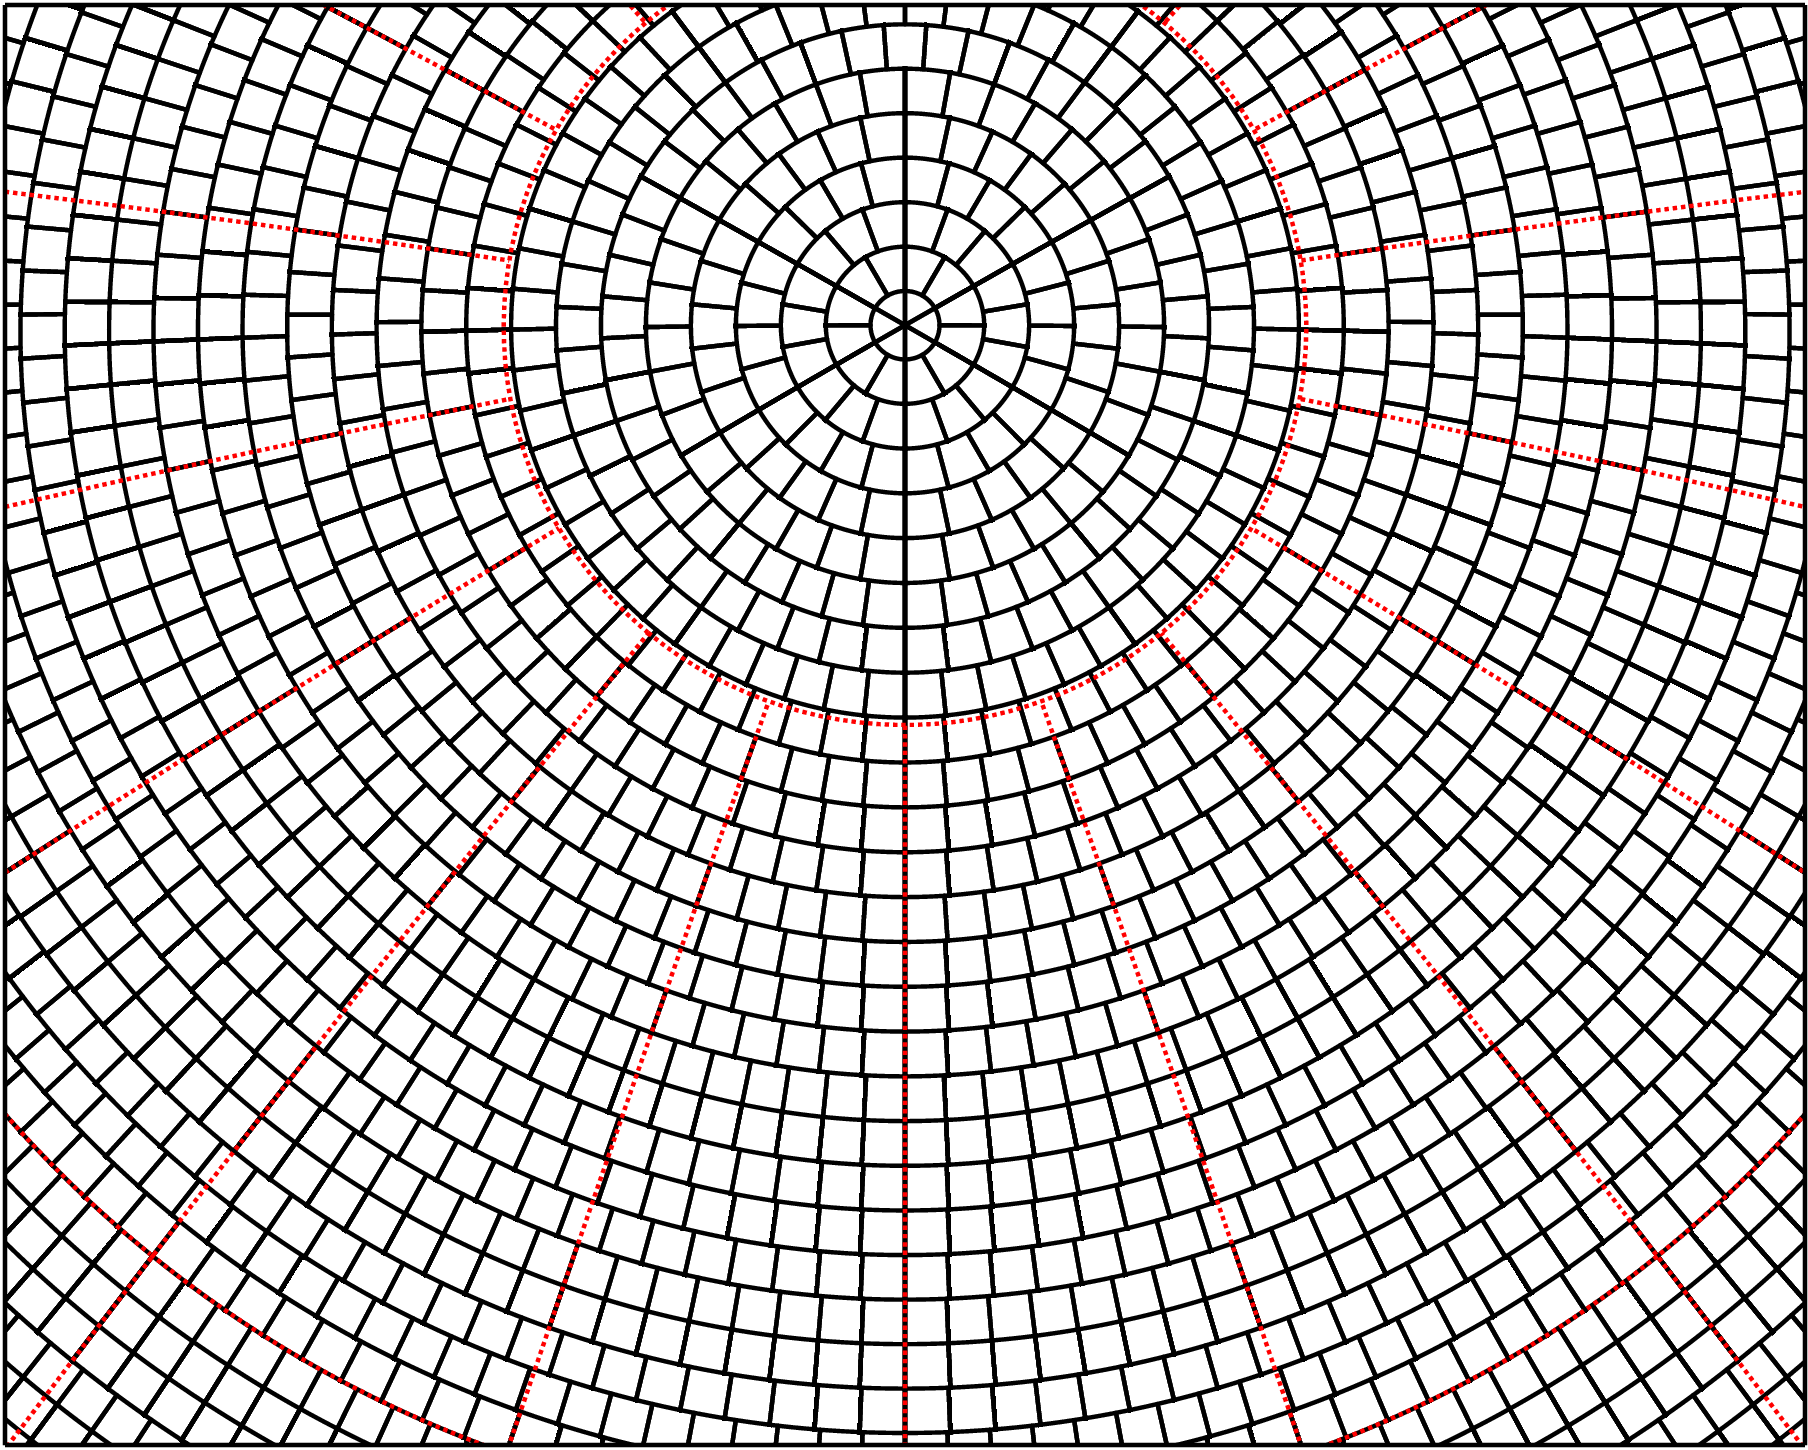
\includegraphics[width=\linewidth]{hortal.png}
    \caption{The "fully" reduced grid by Hortal (reconstructed
      from~\cite{Rasch1994}). As the resolution was too fine, the grid is
      represented with a \gls{Lambert equal-area projection}, centered at latitude
  80\degree. }
    \label{fig:hortal}
  \end{minipage}
  \hfill
\end{figure}
One example of practical use is the dynamical core developed by the \gls{JMA} in
their Global Spectral Model (see~\cite{JMA2013} for more details).

\subsection{Description}
\label{subsubsec:description}
For the grid in Pangolin, we follow the same idea as~\cite{Kurihara1965}: the
cell height is constant and at a given latitude, cell width is constant.
We will show our grid has a very lightweight description: only the number of
latitudes on both hemisphere $N_{lat}$ and the number of cells at the pole $n_1$
are needed.
While~\cite{Kurihara1965} used one grid point for the pole itself, we have
chosen not to have a cell centered on the pole.
It should be noted that, while~\cite{Kurihara1965} set the middle of
its cells at the Equator, we have chosen to place the walls of the cell at the
Equator.
Choosing the number of cells on the first (and last) colatitude is arbitrary.
For our grid, we have chosen to take the regular latitude-longitude grid as a
reference. If we consider square cells at the Equator, as regular
latitude-longitude grid usually have, writing the area preservation formula
leads to $n_1 = 3$ for small latitudinal spacing (see the proof in
Appendix~\ref{sec:pole_area}).

To construct the grid, we only need to consider the Northern hemisphere, as the
Southern hemisphere is its symmetric in respect to the Equator.  We now derive
the formula for the number of cells $n_i$ at colatitude $i$. We no longer
require square cells at the Equator as before. Let us note the cell $(i,j)$ as
being defined on 
$\Omega_{ij} = [\lambda_j, \lambda_{j+1}]\times [\phi_{i-1},\phi_i]$. 
where $\phi_i=i\Delta\phi_i$ is the colatitude and
$\lambda_{ij}=j\Delta\lambda_i$ the longitude.
$\Delta\phi_i$ and $\Delta\lambda_i$ are the latitudinal and
longitudinal spacings respectively.
The area of cell $(i,j)$ is also noted $\mathcal{A}_{i}$, as it does not
depend on $j$. This leads to the following cell area formula in spherical
coordinates:
\begin{equation}
  \mathcal{A}_{i} = \iint_{\Omega_{ij}}  r^2 \sin\phi 
  \mathrm{d}\lambda \mathrm{d}\phi \nonumber
  = r^2 \Delta\lambda_i \big (\cos(\phi_{i-1}) - \cos(\phi_{i-1}+\Delta\phi_i)\big).
  \label{eqn:cell_area}
\end{equation}
Areas are preserved so $\mathcal{A}_i=\mathcal{A}_1$:
\begin{align*} \Delta\lambda_i  = \Delta\lambda_1 \frac {1-\cos(\Delta\phi_1)}
  {2\sin\left( \frac{\Delta\phi_i}{2} \right) \sin\left(\left(i-\frac{1}{2}\right)\Delta\phi_i\right)}.
\end{align*}
The number of cells at colatitude $i$ can be defined by
$n_i = \lfloor \frac{2\pi}{\Delta\Lambda_i}\rfloor$ so:
\begin{align*} \frac{n_i}{n_1} = \left\lfloor \frac{\Delta\lambda_1}{\Delta\lambda_i} \right\rfloor=
  \left\lfloor \frac {2\sin\left( \frac{\Delta\phi_i}{2} \right) \sin\left(\left(i-\frac{1}{2}\right)\Delta\phi_i\right)}%
  {1-\cos(\Delta\phi_1)}\right\rfloor.
\end{align*}
Now let us assume $\forall i$, $\Delta\phi_i$ and
$(i-\frac{1}{2})\Delta\phi_i$ are small enough so the sinus can be approximated
by their angle:
\begin{align*} \frac{n_i}{n_1} \approx
  \left\lfloor \frac{2  \frac{\Delta\phi_i}{2}  \left(i-\frac{1}{2}\right) \Delta\phi_i}%
  { \frac{\Delta\phi_1^2}{2}} \right\rfloor
  = 2i-1.
\end{align*}
If the Southern hemisphere is constructed as the symmetric of the Northern
hemisphere, this leads to:
\begin{align}
  &n_i = nb\_cells(i) =
  \begin{cases}
    3(2i-1) & \quad \text{if} \; 1 \le i \le N_{\text{lat}}/2, \\
    nb\_cells(N_\mathrm{lat}-i+1) & \quad \text{otherwise.}
  \end{cases}
  \label{eqn:nb_cells}
\end{align}
It follows that the total number of cells on the grid is $6N_{\text{lat}}^2$. As
an illustration, the grid is shown on Fig.~\ref{fig:pango_grid}.
\begin{figure}
  \begin{minipage}[t]{0.49\linewidth}
    \centering
    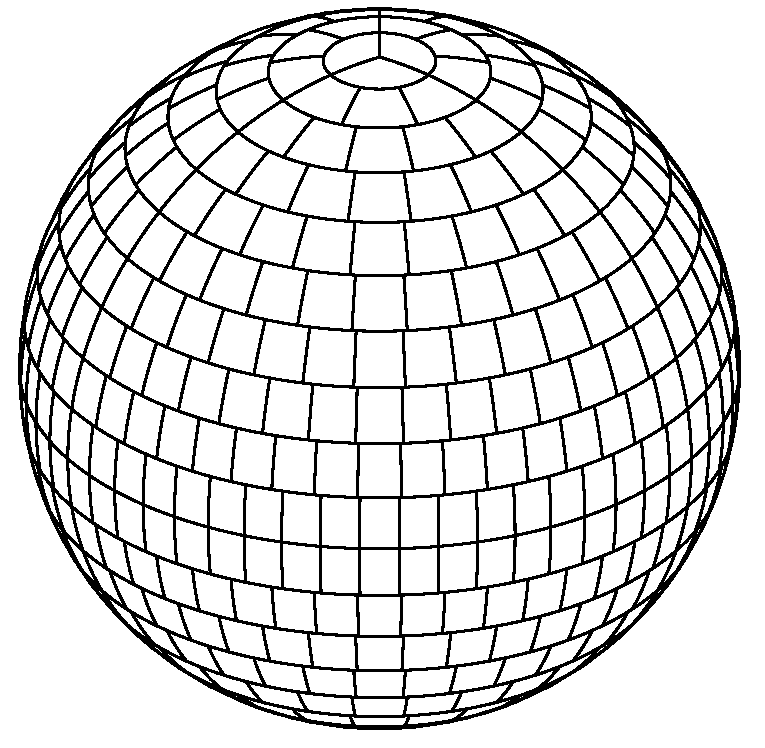
\includegraphics[width=\linewidth]{pangolin.pdf}
    \caption{Pangolin grid with 20 latitudes.}
    \label{fig:pango_grid}
  \end{minipage} 
  \hfill
  \begin{minipage}[t]{0.49\linewidth}
    \centering
    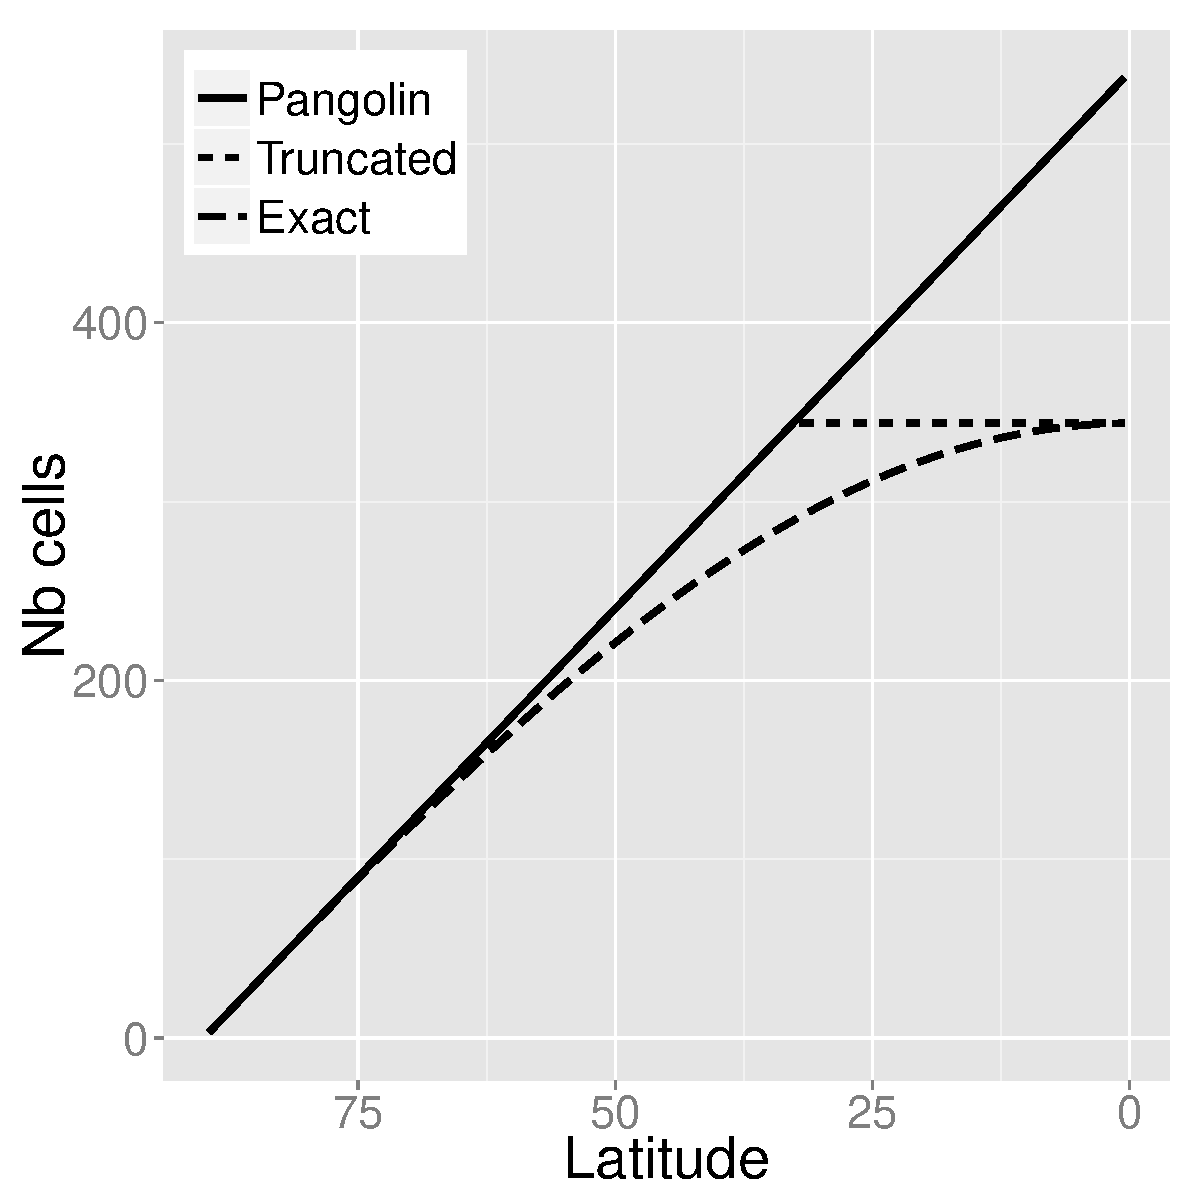
\includegraphics[width=\linewidth]{nb_cells.pdf}
    \caption{
      Comparison of the number of cells on Pangolin for our
      approximation (solid line), the truncated approximation and the ''exact''
    version.  The grid has 90 latitudes on one hemisphere.}
    \label{fig:nb_cells}
  \end{minipage}
\end{figure}

To derived the number of cells in Eq.~\eqref{eqn:nb_cells} from the area
preservation formula, two approximations were made. The first is to consider the
latitudinal spacing small enough, a valid assumption for
resolution of $1^{\circ}$ of latitude. In this case, we only make an error of
only 0.001\% when approximating $\sin(\Delta\phi_i/2)$ by $\Delta\Phi_i/2$ for
all $i$.
The other approximation is to consider that latitudes are close to the North
pole, \textit{i.e}, for all $i$ $(i-1/2)\Delta\phi_i \ll~1$. 
In practice, the relative error is less than 1\% up to to 75\degree but
increases for lower latitudes, with a maximum of 56\% at the Equator. On top of
that, the resolution given by this approximation is higher than it should be at
the Equator. This is illustrated on Fig.~\ref{fig:nb_cells}, where the linear
approximation is compared to the ''exact'' number of cells (\textit{i.e}, without
approximation). One solution to decrease the number of cells at the Equator is
to truncate the number of cells at some point (dashed line on the figure). 
To truly preserve the cell areas, we should also use a variable cell height.
However, the error in the cell area preservation was found to be acceptable so
both of these two possible improvements were not implemented in Pangolin.

\begin{figure}
  \begin{minipage}{0.5\linewidth}
    \centering
    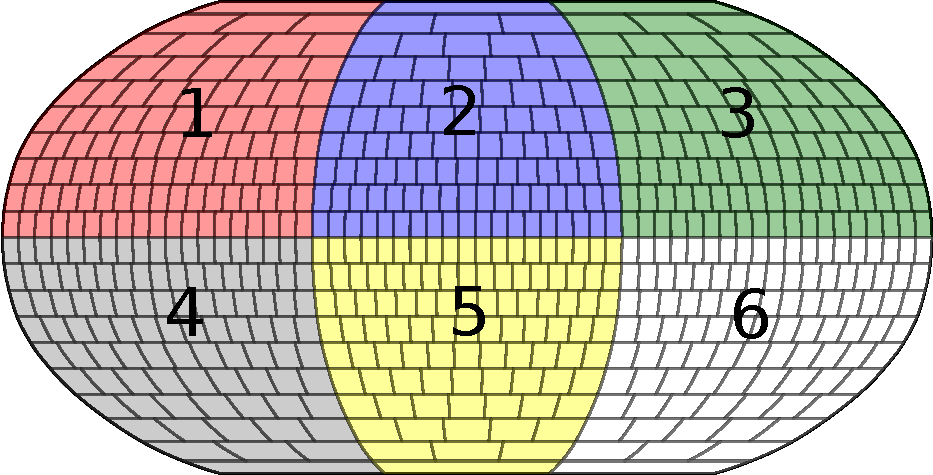
\includegraphics[width=\linewidth]{pangolin_zones.pdf}
    \caption{The six identical zones in the Pangolin grid with 20 latitudes with
      a \gls{Robinson projection}.}
    \label{fig:pango_zones}
  \end{minipage}
  \hfill
  \begin{minipage}{0.4\linewidth}
    \centering
    \includegraphics[width=0.7\linewidth]{discretization.pdf}
    \caption{Discretization of zonal and meridional winds ($u$ and $v$ 
    respectively) and tracer data $q$ for cell $(i,j)$ in Pangolin.}
    \label{fig:d-grid}
  \end{minipage}
\end{figure}

\subsubsection{Neighbours of a cell}
From Fig.~\ref{fig:pango_grid}, it can be seen that, while the Pangolin grid is not
unstructured, computing the meridional neighbours of a cell are not immediate.
On the other hand, zonal neighbours are easily computed. With periodical
boundaries, the zonal neighbours of cell $(i,j)$ are simply:
\begin{equation}
  \begin{cases}
    (i,j-1) \quad \text{if} \; j > 1, \\
    (i, n_i)  \quad \text{otherwise,}
  \end{cases}
  \quad \text{and} \quad
  \begin{cases}
    (i,j+1) \quad \text{if} \; j < n_i, \\
    (i,1)  \quad \text{otherwise.}
  \end{cases}
\end{equation}
To find the meridional neighbour, we have to exploit the symmetries of the grid.
From Eq.~\eqref{eqn:nb_cells}, we can deduce the grid has 4 axes of symmetry:
the Equator and the meridians $\lambda=0$, $120$ and $240^\circ$. The grid can
then be split into six identical zones, as shown on Fig.~\ref{fig:pango_zones}.
In the rest of this paragraph, we only consider the first zone.  For zones 2 and
3, the neighbours are found by adding the proper offset. On the South hemisphere
(zone 4 to 6), north and south neighbours are simply inverted. So the meridional
neighbours on zone 1 for the cell $(i,j)$ are
$\big\{(i-1,j_1), \ldots, (i-1, j_2)\big\}$ (northern) and 
$\big\{(i+1,j_3), \ldots, (i+1, j_4)\big\}$ (southern), with:
\begin{equation}
  \begin{aligned}
    j_1 &= \left\lfloor \frac{n_{i-1}}{n_i}(j-1)+1\right\rfloor, \;
    j_2 = \left\lceil \frac{n_{i-1}}{n_i}j\right\rceil \\
    \text{and} \quad 
    j_3 &= \left\lfloor \frac{n_{i+1}}{n_i}(j-1)+1\right\rfloor, \;
    j_4 = \left\lceil \frac{n_{i+1}}{n_i}j\right\rceil.
    \label{eqn:neighb_merid}
  \end{aligned}
\end{equation}

From Eq.~\eqref{eqn:neighb_merid}, it can be shown that most cells have two
northern neighbours and two southern neighbours. Special cases include:
\begin{itemize}
  \item the center of each zone, where a cell has one (resp.~three) northern
    neighbour(s) and three (resp.~one) southern neighbour(s) on the Northern (resp. Southern
    hemisphere),
  \item the westmost cells on each zone, with one (resp.~two) northern neighbour(s)
    and two (resp.~one) southern neighbour(s) on the Northern (resp. Southern
    hemisphere),
  \item the eastmost cells on each zone, with the same number of neighbours as
    the westmost cells.
\end{itemize}

To decrease memory costs, the neighbours of the cells are not stored, contrary
to unstructured grids, but are computed explicitly when needed.
The computation is efficient as it involves only integer computation with some
rounding. Due to the current trend of decreasing memory per core (see
Section~\ref{subsubsec:paradigms}), we are emphasizing CPU computation to the
expensive of memory. From a more general point-of-view, the algebraic features
of the grid have been exploited as much as possible, especially in the
parallelization process (see Section~\ref{subsec:domain_decompos}).

\subsection{Pangolin and other reduced grids}
While we did not present all reduced grids, we believe the chosen panel is
representative of the different possible choices.  On Table~\ref{tab:reduced} is
shown the gains in the number of cells when using the different reduced grids
presented before as opposed to a regular latitude-longitude grid.  Kurihara's
reduced grid is quite similar to the Pangolin grid but has approximately twice
the number of cells for each latitude. The grid by Rasch
and Hortal has similar gains compared to the Pangolin grid. Rasch's grid
allows for a more efficient computation of the neighbours : it only requires a
distance computed once of every latitude and the neighbours are fewer and
somewhat easier to compute.  Hortal's is less relevant in our case as it is
specifically designed for spectral models. However, if we were to adapt it to a
finite-volume approach, it would require to store the neighbours as for an
unstructured grid, thus increasing memory footprint. The most important requirement
remains its parallel efficiency and the domain decomposition algorithm is an
important aspect. The advantage of Pangolin is its custom algorithm, which
exploits the analytical features as much as possible (see
Section~\ref{subsec:domain_decompos}).

\def\Ast{($^{\ast}$) }
\begin{table}
  \centering
  \caption{Gains of the different reduced grids versus the regular
    latitude-longitude grid. The gains noted \Ast were computed using the
  same resolution at the Equator of $1\degre$ for comparison.}
  \label{tab:reduced}
  \begin{tabular}{lcc}
    \toprule
    Grid & Reference & Gain\\
    \midrule 
    Reduced Gaussian & \cite{Hortal1990} & 34.5\% \\
    Reduced & \cite{Kurihara1965} & 50\% \Ast\\
    Reduced/composite & \cite{Rasch1994} & 34.5\% \Ast \\
    Pangolin & this manuscript & 33\% \Ast\\
   \bottomrule
  \end{tabular}
\end{table}

\subsection{Adapting the scheme to the grid}
To discretize the winds and tracer data, we use the same approach as the D-grid
of~\cite{Arakawa1977}, illustrated on Fig~\ref{fig:d-grid}. In practice, data is
either generated at the proper position in the case of analytical tests
(Chapter~\ref{chap:testing}) or interpolated onto the grid when using "real" data
(Chapter~\ref{chap:real_case}).
\begin{figure}
  \begin{minipage}[t]{0.48\linewidth} 
    \centering
    \includegraphics[width=0.7\linewidth]{merid_fluxes.pdf}
    \caption{ Meridional interfaces (bold lines) and fluxes (dark arrows) for
    cell $(i,j)$.}
    \label{fig:merid_fluxes}
  \end{minipage}
  \hfill
  \begin{minipage}[t]{0.48\linewidth} 
    \centering
    \includegraphics[width=0.7\linewidth]{merid_gradient.pdf}
    \caption{Linear interpolation to compute the meridional gradient.}
    \label{fig:merid_interpol}
  \end{minipage}
\end{figure}

While there is not particular difficulty to compute the zonal fluxes, the varying
number of meridional neighbours means we have to compute the contribution of
each neighbours. In practice, this means we have compute the interface between a
cell and its meridional neighbours. As the neighbours are given by
Eq.~\eqref{eqn:neighb_merid} and knowing that cell width is constant at a given
latitude, the size of the interfaces can be easily computed.
Computing the meridional gradient is also not immediate. We use a linear
interpolation to set a north and south ratio and compute the meridional gradient
with finite-differences, as in Eq.~\eqref{eqn:slope}. The interpolation is shown on
Fig.~\ref{fig:merid_interpol}.
The sequential algorithm for 2D advection is summarized in
Algorithm.~\ref{algo:seq_zonal} and~\ref{algo:seq_merid}. The parallel version is
presented in Section~\ref{subsec:parallel_advection}.
\begin{algorithm}
  \begin{algorithmic}[1]
    \State Compute zonal gradient 
    \State Compute zonal fluxes 
    \State Update ratios
  \end{algorithmic}
  \caption{Sequential zonal advection}
  \label{algo:seq_zonal}
\end{algorithm}
\begin{algorithm}
  \begin{algorithmic}[1]
    \State Compute zonal gradient 
    \State Compute meridional gradient 
    \State Compute meridional fluxes 
    \State Update ratios
  \end{algorithmic}
  \caption{Sequential meridional advection}
  \label{algo:seq_merid}
\end{algorithm}

To ensure mass preservation, winds are corrected such as the winds divergence is
null. For 2D wins, we correct first meridional winds. If we consider a latitude
circle, it constitutes a closed contour and the divergence on it must be null.
So we compute the sum of all meridional fluxes on this circle and subtract the
mean values from all meridional wind such as to achieve a null divergence. Then
zonal winds are corrected such as the sum of all fluxes in each cell is null. To
that end, we browse sequentially all cells at a given latitude and correct each
east wind such as the sum of fluxes is null. The zonal wind at $\lambda=0$ is
used as an initial condition, \textit{i.e}, is not modified by the algorithm.

During a time-step, the tracer mass is updated locally according to the fluxes
in each cell. However, we should avoid unphysical fluxes which empty the
cells of all (or more) of its tracer. This is usually done using a \gls{CFL}
condition. As we use a dimensional splitting algorithms, we have two 1D
\gls{CFL} conditions: one for zonal advection, one for meridional advection. As
a global \gls{CFL}, we use the most restrictive condition in both directions and
for all cells:
\begin{align*} 
  C = \max_{ij} \left(\frac{u_{ij}\Delta t}{\Delta\phi_{ij}},
  \frac{\Delta t\sum_{k \in V_{ij}} v_k \Delta\lambda_k }{
    \Delta\phi_{ij}\sum_{k \in V_{ij}} \Delta\lambda_{k}} \right),
\end{align*}
where $V_{ij}$ is the set of meridional neighbours for the cell
$(i,j)$ and $\Delta\lambda_k$ is the interface size between the
cell and its neighbours.

